\documentclass[twoside,11pt,a4paper,openany]{book}
\usepackage[amsbb,subscriptcorrection,zswash,mtpcal,mtphrb]{mtpro2}
\usepackage[no-math,cm-default]{fontspec}
\usepackage{xunicode}
\usepackage{xgreek}
\defaultfontfeatures{Mapping=tex-text,Scale=MatchLowercase}
\def\xrwma{black}
\def\xrwmath{black}
\setmainfont[Mapping=tex-text,Numbers=Lining,Scale=1.0]{Minion Pro}
\newfontfamily\mpro{Minion Pro}
\font\icon = "Webdings"
\usepackage{fontawesome5}
\usepackage{amsmath}
\usepackage[left=2.00cm, right=2.00cm, top=3.00cm, bottom=2.00cm]{geometry}
\usepackage{makeidx}
\usepackage{longtable}
\usepackage{etoolbox}
\makeatletter
\newif\ifLT@nocaption
\preto\longtable{\LT@nocaptiontrue}
\appto\endlongtable{%
\ifLT@nocaption
\addtocounter{table}{\m@ne}%
\fi}
\preto\LT@caption{%
\noalign{\global\LT@nocaptionfalse}}
\makeatother
\makeindex
\usepackage{tikz,pgfplots}
\usepackage{tkz-euclide}
\usepackage{wrapfig}
\usepackage{calc}
\usepackage[colorlinks=false, pdfborder={0 0 0}]{hyperref}
\usepackage[framemethod=TikZ]{mdframed}
\newcommand{\ypogrammisi}[1]{\underline{\smash{#1}}}
\usetikzlibrary{backgrounds}
\renewcommand{\thepart}{\arabic{part}}
\definecolor{steelblue}{cmyk}{.7,.278,0,.294}
\definecolor{doc}{cmyk}{1,0.455,0,0.569}
\definecolor{olivedrab}{cmyk}{0.25,0,0.75,0.44}
\usepackage{capt-of}
\usepackage{titletoc}
\usepackage[explicit]{titlesec}
\usepackage{graphicx}
\usepackage{multicol}
\usepackage{multirow}
\usepackage{enumitem}
\usepackage{tabularx}
\usepackage{mathimatika,tkz-tab,gensymb}
\tikzset{>=latex}
\makeatletter
\pretocmd{\@part}{\gdef\parttitle{#1}}{}{}
\pretocmd{\@spart}{\gdef\parttitle{#1}}{}{}
\makeatother
\usepackage[titletoc]{appendix}
\usepackage{fancyhdr}
\pagestyle{fancy}
\fancyheadoffset{0cm}
\renewcommand{\headrulewidth}{\iftopfloat{0pt}{.5pt}}
\renewcommand{\chaptermark}[1]{\markboth{#1}{}}
\renewcommand{\sectionmark}[1]{\markright{\it\thesection\ #1}}
\fancyhf{}
\fancyhead[LE]{\thepage\ $\cdot$\ \scshape\nouppercase{\leftmark}}
\fancyhead[RO]{\nouppercase{\rightmark} $\cdot$\ \thepage}
\fancypagestyle{plain}{%
\fancyhead{} %
\renewcommand{\headrulewidth}{0pt}}

\newcounter{thewrhma}[chapter]
\renewcommand{\thethewrhma}{\thechapter.\arabic{thewrhma}} 
\newcommand{\Thewrhma}[1]{\refstepcounter{thewrhma}{\textbf{\textcolor{\xrwmath}{{\large Θεώρημα\hspace{2mm}\thethewrhma\;}:\;}\hspace{1mm}}} \MakeUppercase{\textbf{#1}}\\}{}

\newcounter{porisma}[chapter]
\renewcommand{\theporisma}{\thechapter.\arabic{porisma}}\newcommand{\Porisma}[1]{\refstepcounter{porisma}\textcolor{black}{\textbf{ΠΟΡΙΣΜΑ\hspace{2mm}\theporisma\hspace{1mm} \MakeUppercase{#1}}}\\}{}

\newcounter{protasi}[chapter]
\renewcommand{\theprotasi}{\thechapter.\arabic{protasi}}\newcommand{\Protasi}[1]{\refstepcounter{protasi}\textcolor{black}{\textbf{ΠΡΟΤΑΣΗ\hspace{2mm}\theprotasi\hspace{1mm} \MakeUppercase{#1}}}\\}{}

\newcounter{methodologia}[chapter]
\renewcommand{\themethodologia}{\thechapter.\arabic{methodologia}}\newcommand{\Methodologia}[1]{\refstepcounter{methodologia}\textcolor{black}{\textbf{MΕΘΟΔΟΣ\hspace{2mm}\themethodologia\hspace{1mm} \MakeUppercase{#1}}}\\}{}

\newcounter{orismos}[chapter]
\renewcommand{\theorismos}{\arabic{orismos}}   
\newcommand{\Orismos}[1]{\refstepcounter{orismos}{\textbf{\textbf{\textcolor{\xrwma}{{\large Ορισμός\hspace{2mm}\thechapter.\theorismos\;}:\;}}}}\hspace{1mm} \MakeUppercase{\textbf{#1}\\}}{}
\usepackage{venndiagram}
%-------- ΣΤΥΛ ΚΕΦΑΛΑΙΟΥ ---------
\newcommand*\chapterlabel{}
\newcommand{\fancychapter}{%
\titleformat{\chapter}
{
\normalfont\Huge}
{\gdef\chapterlabel{\thechapter\ }}{0pt}
{\begin{tikzpicture}[remember picture,overlay]
\node[yshift=-7cm] at (current page.north west)
{\begin{tikzpicture}[remember picture, overlay]
%\node[inner sep=0pt] at ($(current page.north) +			(0cm,-1.38in)$) {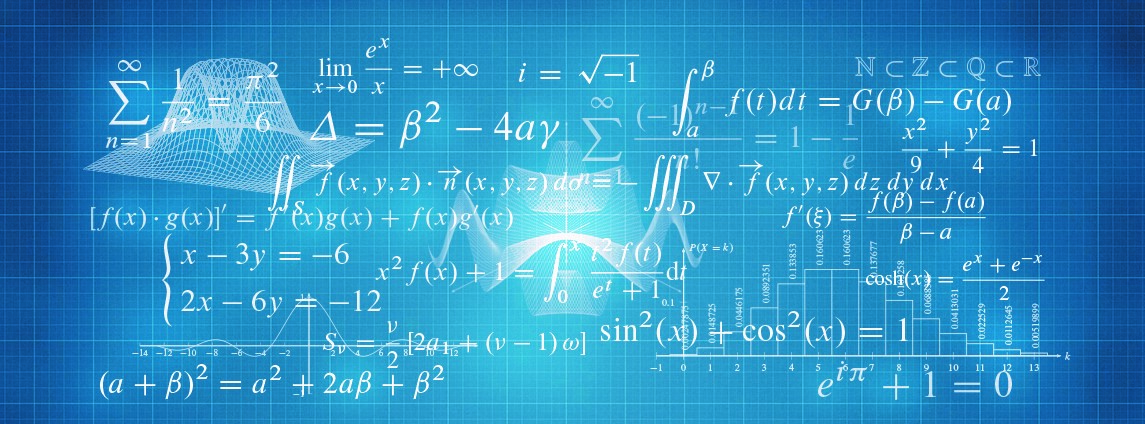
\includegraphics[width=17cm]{Kefalaio}};
\node[anchor=west,xshift=.08\paperwidth,yshift=.1\paperheight,rectangle]
{{\color{white}\fontsize{30}{20}\textbf{\textcolor{black}{\contour{white}{ΚΕΦΑΛΑΙΟ}}}}};
\node[anchor=west,xshift=.07\paperwidth,yshift=.05\paperheight,rectangle] {\fontsize{27}{20} {\color{black}{{\textcolor{black}{\contour{white}{\sc##1}}}}}};
%\fill[fill=black] (12.2,2) rectangle (14.8,4.7);
\node[anchor=west,xshift=.77\paperwidth,yshift=.077\paperheight,rectangle]
{\fontsize{80}{20}\textbf{\textit{\contour{black}{\thechapter}}}};
\end{tikzpicture}
};
\end{tikzpicture}
}
\titlespacing*{\chapter}{0pt}{20pt}{30pt}
}
%------------------------------------------------

\usepackage[outline]{contour}
\newcommand{\regularchapter}{%
\titleformat{\chapter}[display]
{\normalfont\huge\bfseries}{\chaptertitlename\ \thechapter}{20pt}{\Huge##1}
\titlespacing*{\chapter}
{0pt}{-20pt}{40pt}
}

\apptocmd{\mainmatter}{\fancychapter}{}{}
\apptocmd{\backmatter}{\regularchapter}{}{}
\apptocmd{\frontmatter}{\regularchapter}{}{}

\titlespacing*{\section}
{0pt}{30pt}{0pt}
\usepackage{booktabs}
\usepackage{hhline}
\DeclareRobustCommand{\perthousand}{%
\ifmmode
\text{\textperthousand}%
\else
\textperthousand
\fi}

\newcounter{typos}[chapter]
\renewcommand{\thetypos}{T\arabic{typos}}   
\newcommand{\Typos}{\refstepcounter{typos}\textcolor{gray}{\textbf{\thetypos}}}{}


\contentsmargin{0cm}
\titlecontents{part}[-1pc]
{\addvspace{10pt}%
\bf\Large ΜΕΡΟΣ\quad }%
{}
{}
{\;\dotfill\;\normalsize\ Σελίδα}%
%------------------------------------------
\titlecontents{chapter}[0pc]
{\addvspace{30pt}%
\begin{tikzpicture}[remember picture, overlay]%
\draw[fill=black,draw=black] (-.3,.5) rectangle (3.7,1.1); %
\pgftext[left,x=0cm,y=0.75cm]{\color{white}\sc\Large\bfseries Κεφάλαιο\ \thecontentslabel};%
\end{tikzpicture}\large\sc}%
{}
{}
{\hspace*{-2.3em}\hfill\normalsize Σελίδα \thecontentspage}%
\titlecontents{section}[2.4pc]
{\addvspace{1pt}}
{\contentslabel[\thecontentslabel]{2pc}}
{}
{\;\dotfill\;\small \thecontentspage}
[]
\titlecontents*{subsection}[4pc]
{\addvspace{-1pt}\small}
{}
{}
{\ --- \small\thecontentspage}
[ \textbullet\ ][]

\makeatletter
\renewcommand{\tableofcontents}{%
\chapter*{%
\vspace*{-20\p@}%
\begin{tikzpicture}[remember picture, overlay]%
\pgftext[right,x=12cm,y=0.2cm]{\Huge\sc\bfseries \contentsname};%
\draw[fill=black,draw=black] (9.5,-.75) rectangle (12.5,1);%
\clip (9.5,-.75) rectangle (15,1);
\pgftext[right,x=12cm,y=0.2cm]{\color{white}\Huge\bfseries \contentsname};%
\end{tikzpicture}}%
\@starttoc{toc}}
\makeatother
\pgfmathdeclarefunction{gauss}{2}{%
\pgfmathparse{1/(#2*sqrt(2*pi))*exp(-((x-#1)^2)/(2*#2^2))}%
}
\usepackage[contents={},scale=1,opacity=1,color=black,angle=0]{background}

\newcommand\blfootnote[1]{%
\begingroup
\renewcommand\thefootnote{}\footnote{#1}%
\addtocounter{footnote}{-1}%
\endgroup
}
\usepackage{epstopdf}
\epstopdfsetup{update}
\usepackage{textcomp}
\titleformat{\section}
{\normalfont\Large\bf}%
{}{0em}%
{{\color{black}\titlerule[1pt]}\vskip-.2\baselineskip{\parbox[t]{\dimexpr\textwidth-2\fboxsep\relax}{\raggedright\strut\thesection~#1\strut}}}[\vskip 0\baselineskip{\color{black}\titlerule[1pt]}]
\titlespacing*{\section}{0pt}{0pt}{0pt}

\newcommand{\methodologia}{\begin{center}
{\large \textbf{ΜΕΘΟΔΟΛΟΓΙΑ}}\\\vspace{-2mm}
\begin{tikzpicture}
\shade[left color=white, right color=black] (-3cm,0) rectangle (0,.2mm);
\shade[left color=black, right color=white] (0,0) rectangle (3cm,.2mm);   
\end{tikzpicture}
\end{center}}

\newcommand{\orismoi}{\begin{center}
\large \textcolor{\xrwma}{\textbf{ΟΡΙΣΜΟΙ}}\\\vspace{-2mm}
\begin{tikzpicture}
\shade[left color=white, right color=\xrwma] (-3cm,0) rectangle (0,.2mm);
\shade[left color=\xrwma, right color=white] (0,0) rectangle (3cm,.2mm);   
\end{tikzpicture}
\end{center}}
\newcommand{\thewrhmata}{\begin{center}
{\large \textcolor{\xrwmath}{\textbf{ΘΕΩΡΗΜΑΤΑ - ΠΟΡΙΣΜΑΤΑ - ΠΡΟΤΑΣΕΙΣ\\ΚΡΙΤΗΡΙΑ - ΙΔΙΟΤΗΤΕΣ}}}\\\vspace{-2mm}
\begin{tikzpicture}
\shade[left color=white, right color=\xrwmath,] (-5cm,0) rectangle (0,.2mm);
\shade[left color=\xrwmath, right color=white,] (0,0) rectangle (5cm,.2mm);   
\end{tikzpicture}
\end{center}}
\usepackage[labelfont={footnotesize,it,bf},font={footnotesize}]{caption}

\usepackage{wrapfig,wrap-rl}
%-------- ΜΑΘΗΜΑΤΙΚΑ ΕΡΓΑΛΕΙΑ ---------
\usepackage{mathtools}
%----------------------
%-------- ΠΙΝΑΚΕΣ ---------
\usepackage{booktabs}
%----------------------
%----- ΥΠΟΛΟΓΙΣΤΗΣ ----------
%\usepackage{calculator}
%----------------------------
\newcommand{\tss}[1]{\textsuperscript{#1}}
\newcommand{\tssL}[1]{\MakeLowercase{\textsuperscript{#1}}}
%----- ΟΡΙΖΟΝΤΙΑ ΛΙΣΤΑ ------
\usepackage{xparse}
\newcounter{answers}
\renewcommand\theanswers{\arabic{answers}}
\ExplSyntaxOn
\NewDocumentCommand{\results}{m}
{
\seq_set_split:Nnn \l_results_a_seq {,}{#1}
\par\nobreak\noindent\setcounter{answers}{0}
\seq_map_inline:Nn \l_results_a_seq
{
\makebox[.18\linewidth][l]{\stepcounter{answers}\theanswers.~##1}\hfill
}
\par
}
\seq_new:N \l_results_a_seq
\ExplSyntaxOff
%----------------------------

\usepackage{microtype}
\usepackage{float}
\usepackage{caption}
%----------- ΓΡΑΦΙΚΕΣ ΠΑΡΑΣΤΑΣΕΙΣ ---------
\pgfkeys{/pgfplots/aks_on/.style={axis lines=center,
xlabel style={at={(current axis.right of origin)},xshift=1.5ex, anchor=center},
ylabel style={at={(current axis.above origin)},yshift=1.5ex, anchor=center}}}
\pgfkeys{/pgfplots/grafikh parastash/.style={\xrwma,line width=.4mm,samples=200}}
\pgfkeys{/pgfplots/belh ar/.style={tick label style={font=\scriptsize},axis line style={-latex}}}
%-----------------------------------------

%---- ΟΡΙΖΟΝΤΙΟ - ΚΑΤΑΚΟΡΥΦΟ - ΠΛΑΓΙΟ ΑΓΚΙΣΤΡΟ ------
\newcommand{\orag}[3]{\node at (#1)
{$ \overcbrace{\rule{#2mm}{0mm}}^{{\scriptsize #3}} $};}

\newcommand{\kag}[3]{\node at (#1)
{$ \undercbrace{\rule{#2mm}{0mm}}_{{\scriptsize #3}} $};}

\newcommand{\Pag}[4]{\node[rotate=#1] at (#2)
{$ \overcbrace{\rule{#3mm}{0mm}}^{{\rotatebox{-#1}{\scriptsize$#4$}}}$};}
%-----------------------------------------
\tikzstyle{pl}=[line width=0.3mm]
\tikzstyle{plm}=[line width=0.4mm]
\tkzSetUpPoint[size=2.7,fill=white]
\newlist{rlist}{enumerate}{3}
\setlist[rlist]{itemsep=0mm,label=\roman*.}
\setlist[itemize]{itemsep=0mm}
\definecolor{bblue}{HTML}{4F81BD}
\definecolor{rred}{HTML}{C0504D}
\definecolor{ggreen}{HTML}{9BBB59}
\definecolor{ppurple}{HTML}{9F4C7C}

\makeatletter
\usetikzlibrary{patterns}
\tikzstyle{chart}=[
legend label/.style={font={\scriptsize},anchor=west,align=left},
legend box/.style={rectangle, draw, minimum size=5pt},
axis/.style={black,semithick,->},
axis label/.style={anchor=east,font={\tiny}},
]

\tikzstyle{bar chart}=[
chart,
bar width/.code={
\pgfmathparse{##1/2}
\global\let\bar@w\pgfmathresult
},
bar/.style={very thick, draw=white},
bar label/.style={font={\bf\small},anchor=north},
bar value/.style={font={\footnotesize}},
bar width=.75,
]

\tikzstyle{pie chart}=[
chart,
slice/.style={line cap=round, line join=round,thick,draw=white},
pie title/.style={font={\bf}},
slice type/.style 2 args={
##1/.style={fill=##2},
values of ##1/.style={}
}
]

\pgfdeclarelayer{background}
\pgfdeclarelayer{foreground}
\pgfsetlayers{background,main,foreground}


\newcommand{\pie}[3][]{
\begin{scope}[#1]
\pgfmathsetmacro{\curA}{90}
\pgfmathsetmacro{\r}{1}
\def\c{(0,0)}
\node[pie title] at (90:1.3) {#2};
\foreach \v/\s/\l in{#3}{
\pgfmathsetmacro{\deltaA}{\v/100*360}
\pgfmathsetmacro{\nextA}{\curA + \deltaA}
\pgfmathsetmacro{\midA}{(\curA+\nextA)/2}

\path[slice,\s] \c
-- +(\curA:\r)
arc (\curA:\nextA:\r)
-- cycle;
\pgfmathsetmacro{\d}{max((\deltaA * -(.5/50) + 1) , .5)}

\begin{pgfonlayer}{foreground}
\path \c -- node[pos=\d,pie values,values of \s]{$\l$} +(\midA:\r);
\end{pgfonlayer}

\global\let\curA\nextA
}
\end{scope}
}

\newcommand{\legend}[2][]{
\begin{scope}[#1]
\path
\foreach \n/\s in {#2}
{
++(0,-10pt) node[\s,legend box] {} +(5pt,0) node[legend label] {\n}
}
;
\end{scope}
}
\definecolor{a}{cmyk}{0,1,1,0.05}
\definecolor{b}{cmyk}{0,.8,.8,.15}
\definecolor{c}{cmyk}{0,.8,.8,.0}
\definecolor{d}{cmyk}{0,.7,.7,0}
\definecolor{e}{cmyk}{0,.5,.5,0}


\pgfplotsset{every axis/.append style={
x tick label style={/pgf/number format/.cd, 1000 sep={.}}}}
\newcommand{\shmeio}[2]{
\foreach \a in {1,...,#2}{
\node[dot] at (#1+.5,\a/2-.2){};}}


\newfontfamily\scfont{GFS Artemisia}
\font\mymath = "MyMathSymbols"
\newcommand{\titlos}[3]{
\begin{center}
{\begin{figure}[h]
\centering
\includegraphics[width=0.4\linewidth]{C:/texlive/texmf-local/tex/latex/local/frontisthrio/LogotypoFilomatheia1.eps}\ \ \ \ \  
\end{figure}}\vspace{-3mm}

\rule{14.7cm}{.1mm}\\
\vspace{2mm}
ΣΗΜΕΙΩΣΕΙΣ ΜΑΘΗΜΑΤΟΣ - ΘΕΩΡΙΑ, ΜΕΘΟΔΟΛΟΓΙΑ ΚΑΙ ΛΥΜΕΝΕΣ ΑΣΚΗΣΕΙΣ\\
\vspace{1mm}
{\bf\today}\\
\vspace{1mm}
ΤΜΗΜΑ: ΜΑΘΗΜΑΤΙΚΩΝ\\
\vspace{1mm}
ΚΑΘΗΓΗΤΗΣ: ΣΠΥΡΟΣ ΦΡΟΝΙΜΟΣ
\end{center}
\vspace{.5cm}
\begin{center}
{\Large\bf\MakeUppercase{#1}}
\end{center}
\begin{center}
\textbf{{\Huge \textcolor{black}{#2}}}
\end{center}
\vspace{-1mm}
\begin{center}
{\Large\bf{\MakeUppercase{#3}}}
\end{center}
\vspace{1cm}}

%--------- tkz-tab Πίνακες --------
\makeatletter
\xpatchcmd{\tkzTabLine}
{\node at (Z\thetkz@cnt@impair\thetkz@cnt@lg){$0$};} % search
{\node[fill=white,inner sep=.5mm] at (Z\thetkz@cnt@impair\thetkz@cnt@lg){$0$};} % replace
{}{}
\makeatother
%----------------------------------


%------ ΕΝΑΡΞΗ ΚΕΙΜΕΝΟΥ ----------
\begin{document}
\pagenumbering{gobble}% Remove page numbers (and reset to 1)
\clearpage
\backmatter
\pagestyle{empty}
\titlos{Α΄ ΛΥΚΕΙΟΥ}{Αλγεβρα}{Ορισμοί και θεωρήματα}
\vspace{1cm}
\begin{center}
\begin{tikzpicture}
\begin{axis}[opacity=.5,aks_on,belh ar,xlabel={\footnotesize$x$},ylabel={\footnotesize$y$}
,xmin=-3,xmax=3.2,ymin=-3,ymax=3.2,x=1cm,y=1cm]
\addplot[opacity=.5,domain=-2:2,grafikh parastash]{x^2-1.4};
\addplot[opacity=.5,domain=-2:2,grafikh parastash]{x^2-2.2};
\end{axis}
\node at (1,2) {$x^2-Sx+p=0$};
\node at (5.5,4) {$P(A\cup B)=P(A)+P(B)-P(A\cap B)$};
\node at (-0.5,1) {$x_{1,2}=\dfrac{-\beta\pm\sqrt{\varDelta}}{2a}$};
\node at (5.5,1) {$|x|=\ccases{x & x\geq0\\-x & x<0}$};
\node at (0.5,5) {$S_\nu=\dfrac{\nu}{2}\left[2a_1+(\nu-1)\cdot\omega\right]$};
\node at (0,3.5) {$\sqrt[\nu]{a^\mu}=a^{\frac{\mu}{\nu}}$};
\node at (5.5,5.5) {$a_{\nu}=a_1\cdot\lambda^{\nu-1}$};
\node at (3.5,2.5) {$ \mathbb{Q}=\left\lbrace \left. \frac{a}{\beta}\right|a,\beta\in\mathbb{Z},\beta\neq0\;\right\rbrace  $};
\end{tikzpicture}\mbox{}\\
\vspace{3cm}
\begin{minipage}{7cm}
\begin{center}
ΑΝΑΛΥΤΙΚΟ ΤΥΠΟΛΟΓΙΟ ΓΙΑ ΤΗ ΘΕΩΡΙΑ ΤΗΣ ΑΛΓΕΒΡΑΣ Α΄ ΛΥΚΕΙΟΥ
\end{center}
\end{minipage}
\end{center}
\vspace*{\fill{\begin{center}
\end{center}}}
\newpage\phantom{}
\vspace{7cm}
\begin{center}
\begin{flushright}
\begin{minipage}{7cm}
\textit{Αεί ο Θεός ο Μέγας γεωμετρεί,
το κύκλου μήκος ίνα ορίση διαμέτρω,
παρήγαγεν αριθμόν απέραντον,
καί όν, φεύ,
ουδέποτε όλον θνητοί θα εύρωσι.}
\[ \pi=3{,}1415926535897932384626 \]
Το πλήθος των γραμμάτων κάθε λέξης στην παραπάνω πρόταση φτιάχνουν διαδοχικά τα 23 πρώτα ψηφία του αριθμού $ \pi $.
\end{minipage}
\end{flushright}
\end{center}
\pagenumbering{arabic}
\mainmatter
\pagestyle{fancy}
\chapter{Σύνολα}
\section{Η έννοια του συνόλου}\mbox{}\\
\orismoi
\Orismos{Σύνολο} 
Σύνολο ονομάζεται μια συλλογή όμοιων αντικειμένων, τα οποία είναι καλά ορισμένα και διακριτά μεταξύ τους.
\begin{itemize}[itemsep=0mm]
\item Τα αντικείμενα ενός συνόλου ονομάζονται \textbf{στοιχεία}.
\item Τα σύνολα τα συμβολίζουμε με ένα κεφαλαίο γράμμα.
\item Για να δηλώσουμε ότι ένα στοιχείο $ x $ \textbf{ανήκει} σε ένα σύνολο $ A $ γράφουμε $ x\in A $. Ενώ αν το $ x $ \textbf{δεν ανήκει} στο σύνολο $ A $ γράφουμε $ x\notin A $.
\item \textbf{Κενό} ονομάζεται το σύνολο που δεν έχει στοιχεία. Συμβολίζεται με $ \varnothing $ ή $ \left\lbrace \right\rbrace  $.
\item \textbf{Βασικό} ονομάζεται το σύνολο που περιέχει όλα τα στοιχεία στο χώρο στον οποίο εργαζόμαστε. Συμβολίζεται $ \varOmega $.
\end{itemize}\mbox{}\\
\textbf{ΒΑΣΙΚΑ ΣΥΝΟΛΑ ΑΡΙΘΜΩΝ}
\begin{enumerate}[itemsep=0mm,label=\bf\arabic*.]
\item \textbf{Φυσικοί Αριθμοί} : Οι αριθμοί $ 0,1,2,\ldots $. Το σύνολο συμβολίζεται με $ \mathbb{N} $ και είναι : $ \mathbb{N}=\{0,1,2,\ldots\} $.
\item \textbf{Ακέραιοι Αριθμοί} : Το σύνολο των φυσικών αριθμών μαζί με τους αντίθετους τους. Συμβολίζεται με $ \mathbb{Z} $ και είναι : $ \mathbb{Z}=\{\ldots,-2,-1,0,1,2,\ldots\} $.
\item \textbf{Ρητοί Αριθμοί} : Όλοι οι αριθμοί που μπορούν να γραφτούν με τη μορφή κλάσματος με ακέραιους όρους. Συμβολίζεται με $ \mathbb{Q} $ και είναι : $ \mathbb{Q}=\left\lbrace \left. \frac{a}{\beta}\right|a,\beta\in\mathbb{Z},\beta\neq0\;\right\rbrace  $.
\item \textbf{Άρρητοι Αριθμοί} : Κάθε αριθμός ο οποίος δεν είναι ρητός. Κατά κύριο λόγο, άρρητοι αριθμοί είναι οι ρίζες που δεν έχουν ρητό αποτέλεσμα, ο αριθμός $ \pi $ κ.τ.λ.
\item \textbf{Πραγματικοί Αριθμοί} : Οι ρητοί μαζί με το σύνολο των άρρητων μας δίνουν τους πραγματικούς αριθμούς, όλους τους αριθμούς που γνωρίζουμε. Συμβολίζεται με $ \mathbb{R} $ και είναι : $ \mathbb{R}= $ $ \{ $όλοι οι αριθμοί$ \} $.
\end{enumerate}
Τα παραπάνω σύνολα \textbf{χωρίς το μηδενικό τους στοιχείο} συμβολίζονται αντίστοιχα με $ \mathbb{N}^*,\mathbb{Z}^*,\mathbb{Q}^*,\mathbb{R}^*$.\\\\
\Orismos{Ίσα σύνολα} Ίσα ονομάζονται δύο σύνολα $ A,B $ τα οποία έχουν ακριβώς τα ίδια στοιχεία. Συμβολίζεται $ A=B $. Ισοδύναμα, τα σύνολα $ Α,Β $ λέγονται ίσα εάν ισχύουν οι σχέσεις :
\begin{enumerate}[itemsep=0mm]
\item Κάθε στοιχείο του $ A $ είναι και στοιχείο του $ B $
\item Κάθε στοιχείο του $ B $ είναι και στοιχείο του $ A $.
\end{enumerate}
\Orismos{Υποσύνολο} Ένα σύνολο $ A $ λέγεται υποσύνολο ενός συνόλου $ B $ όταν κάθε στοιχείο του $ A $ είναι και στοιχείο του $ B $. Συμβολίζεται με τη χρήση του συμβόλου $ \subseteq $ ως εξής : $ A\subseteq B $.\\\\
\Orismos{Παράσταση συνόλου}
Οι τρόποι με τους οποίους μπορούμε να παραστήσουμε ένα σύνολο είναι οι εξής :
\begin{enumerate}[label=\bf\arabic*.]
\item \textbf{Αναγραφή}\\
Γράφουμε τα στοιχεία ενός συνόλου μέσα σε άγκιστρα : $ \{\,\,\} $ όπου κάθε στοιχείο αναγράφεται μια φορά.
\[ A=\{a_1,a_2,\ldots,a_\nu\} \]
Τα στοιχεία του συνόλου χωρίζονται με κομμα (,).
\item \textbf{Περιγραφή}\\
Γράφουμε που ανήκουν τα στοιχεία και ποιά ιδιότητα έχουν. Έχει τη μορφή: $ A=\{x\in\varOmega\;|\;\textrm{Ιδιότητα }I\} $.
\item \textbf{Διάγραμμα Venn}\\
\wrapr{-4mm}{5}{2.5cm}{-15mm}{\begin{tikzpicture}[scale=.5]
\draw(-2,-2) rectangle (2.6,1);
\scope % A \cap B
\fill[\xrwma!30] (-.45,-.5) circle (1.1);
\draw[black] (-.45,-.5) circle (1.1);
\endscope
\tkzText(-1.6,-1.6){$ \varOmega $}
\tkzText(-.45,.2){$ A $}
\end{tikzpicture}}{
Σχεδιάζουμε με ορθογώνιο το βασικό σύνολο και με κύκλους τα υποσύνολά του.}\mbox{}\\
\end{enumerate}
\Orismos{Πράξεισ μεταξύ συνόλων}
\vspace{-5mm}
\begin{enumerate}[label=\bf\arabic*.,itemsep=0mm]
\item \textbf{Ένωση}\\
\begin{minipage}{\linewidth}
\begin{WrapText1}{8}{3.5cm}
\vspace{-5mm}
\begin{venndiagram2sets}[tikzoptions={scale=.7,samples=100},shade=\xrwma!30,labelNotAB={$ \varOmega $}]
\fillA \fillB
\end{venndiagram2sets}
\end{WrapText1}
Ένωση δύο υποσυνόλων $ A,B $ ενός βασικού συνόλου $ \varOmega $ ονομάζεται το σύνολο των στοιχείων του $ \varOmega $ τα οποία ανήκουν σε \textbf{τουλάχιστον ένα} από τα σύνολα $ A $ και $ B $. Συμβολίζεται με $ A\cup B $.  \[ A\cup B=\left\lbrace x\in\varOmega\left| x\in A \textrm{ ή } x\in B\right.\right\rbrace \]
Η ένωση των συνόλων $ A $ και $ B $ περιέχει όλα τα στοιχεία των δύο συνόλων. Τα κοινά στοιχεία αναγράφονται μια φορά.\end{minipage}
\item \textbf{Τομή}\\
\begin{minipage}{\linewidth}
\begin{WrapText1}{7}{3.5cm}
\vspace{-5mm}
\begin{venndiagram2sets}[tikzoptions={scale=.7},shade=\xrwma!30,labelNotAB={$ \varOmega $}]
\fillACapB
\end{venndiagram2sets}
\end{WrapText1}
Τομή δύο υποσυνόλων $ A,B $ ενός βασικού συνόλου $ \varOmega $ ονομάζεται το σύνολο των στοιχείων του $ \varOmega $ τα οποία ανήκουν \textbf{και στα δύο} σύνολα $ A $ και $ B $. Συμβολίζεται με $ A\cap B $. \[ A\cap B=\left\lbrace x\in\varOmega\left| x\in A \textrm{ και } x\in B\right.\right\rbrace \]
Η τομή των συνόλων $ A $ και $ B $ περιέχει μόνο τα κοινά στοιχεία των δύο συνόλων.\end{minipage}
\item \textbf{Συμπλήρωμα}\\
\begin{minipage}{\linewidth}
\begin{WrapText1}{8}{3.5cm}
\vspace{-5mm}
\begin{tikzpicture}[scale=.77]
\filldraw[fill=\xrwma!30] (-2,-2) rectangle (2.6,1);
\scope % A \cap B
\fill[white] (-.45,-.5) circle (1.1);
\draw[black] (-.45,-.5) circle (1.1);
\endscope
\tkzText(-1.6,-1.6){$ \varOmega $}
\tkzText(-.45,.3){$ A $}
\end{tikzpicture}
\end{WrapText1}
Συμπλήρωμα ενός συνόλου $ A $ ονομάζεται το σύνολο των στοιχείων του βασικού συνόλου $ \varOmega $ τα οποία \textbf{δεν} ανήκουν στο $ A $. Συμβολίζεται με $ A' $. \[ A'=\left\lbrace x\in\varOmega\left| x\notin A\right.\right\rbrace \] Ονομάζεται συμπλήρωμα του $ Α $ γιατί η ένωσή του με το σύνολο αυτό μας δίνει το βασικό σύνολο $ \varOmega $.\end{minipage}
\item \textbf{Διαφορά}\\
\begin{minipage}{\linewidth}
\begin{WrapText1}{8}{3.5cm}
\vspace{-5mm}
\begin{venndiagram2sets}[tikzoptions={scale=.7},shade=\xrwma!30,labelNotAB={$ \varOmega $}]
\fillANotB
\end{venndiagram2sets}
\end{WrapText1}
Διαφορά ενός συνόλου $ B $ από ένα σύνολο $ A $ ονομάζεται το σύνολο των στοιχείων του βασικού συνόλου $ \varOmega $ τα οποία ανήκουν \textbf{μόνο} στο σύνολο $ A $, το πρώτο σύνολο της διαφοράς. Συμβολίζεται με $ A-B $. \[ A-B=\left\lbrace x\in\varOmega\left| x\in A\textrm{ και }x\notin B\right. \right\rbrace  \]
\end{minipage}
\end{enumerate}\mbox{}\\\\
\thewrhmata
\Thewrhma{Ιδιότητεσ Υποσυνολου}
Για οποιαδήποτε σύνολα $ A,B,\varGamma $ ισχύουν οι ακόλουθες ιδιότητες που αφορούν τη σχέση του υποσυνόλου :
\begin{rlist}
\item Για κάθε σύνολο $ A $ ισχύει : $ A\subseteq A $.
\item Αν $ A\subseteq B $ και $ B\subseteq \varGamma $ τότε $ A\subseteq \varGamma $.
\item Αν $ A\subseteq B $ και $ B\subseteq A $ τότε $ A=B $.
\end{rlist}
\chapter{Πραγματικοί Αριθμοί}
\section{Πραγματικοί αριθμοί}\mbox{}\\
\orismoi
\Orismos{Άξονασ των πραγματικών αριθμών}
Ο άξονας των πραγματικών αριθμών είναι μια αριθμημένη ευθεία στην οποία μπορούν να τοποθετηθούν όλοι οι πραγματικοί αριθμοί σε αύξουσα σειρά από τα αριστερά προς τα δεξιά. \textbf{Αρχή} του άξονα είναι το σημείο $ O $ στο οποίο βρίσκεται ο αριθμός $ 0 $.
\begin{center}
\begin{tikzpicture}
\tkzInit[xmin=-4,xmax=4]
\draw[-latex] (-5,0) -- coordinate (x axis mid) (5.4,0) node[right,fill=white] {{\footnotesize $ x $}};
\foreach \x in {-5,-4,-3,...,5}
\draw (\x,.5mm) -- (\x,-.5mm) node[anchor=north,fill=white] {{\scriptsize \x}};
\draw[latex-|] (-5,0.7) --  (-0.02,0.7);
\draw[|-latex] (0.02,0.7) --  (5,0.7);
\tkzText(-2,0.85){Αρνητικοί Αριθμοί}
\tkzText(2,0.85){Θετικοί Αριθμοί}
\tkzDefPoint(3,0){A}
\tkzDefPoint(1.4142,0){B}
\tkzDefPoint(-1.5,0){C}
\tkzDefPoint(-2.7,0){D}
\tkzDrawPoints[size=7,fill=white](A,B,C,D)
\tkzLabelPoint[above](A){{\scriptsize $ A(3) $}}
\tkzLabelPoint[above](B){{\scriptsize $ B\left(\!\! \sqrt{2}\right)  $}}
\tkzLabelPoint[above](C){{\scriptsize $ \varGamma\left(-\frac{3}{2} \right)  $}}
\tkzLabelPoint[above](D){{\scriptsize $ \varDelta(-2{,}7) $}}
\end{tikzpicture}
\end{center}
\begin{itemize}[itemsep=0mm]
\item Η θέση ενός αριθμού πάνω στην ευθεία σχεδιάζεται με ένα σημείο.
\item Ο αριθμός που βρίσκεται στη θέση αυτή ονομάζεται \textbf{τετμημένη} του σημείου.
\end{itemize}
\Orismos{Δύναμη πραγματικου αριθμου}
Δύναμη ενός πραγματικού αριθμού $ a $ ονομάζεται το γινόμενο $ \nu $ ίσων παραγόντων του αριθμού αυτού. Συμβολίζεται με $ a^\nu $ όπου $ \nu\in\mathbb{N} $ είναι το πλήθος των ίσων παραγόντων. 
\[ \undercbrace{a\cdot a\cdot\ldots a}_{\nu\textrm{ παράγοντες }}=a^\nu \]
Ο αριθμός $ a $ ονομάζεται \textbf{βάση} και ο αριθμός $ \nu $ \textbf{εκθέτης} της δύναμης.\\\\
\Orismos{ΤΑΥΤΌΤΗΤΑ}
Ταυτότητα ονομάζεται κάθε ισότητα που περιέχει μεταβλητές και επαληθεύεται για κάθε τιμή των μεταβλητών. Παρακάτω βλέπουμε τις βασικές ταυτότητες.
\begin{multicols}{2}
\begin{enumerate}[itemsep=0mm,label=\bf\arabic*.]
\item \parbox[t]{7cm}{\textbf{Άθροισμα στο τετράγωνο}\\$ (a+\beta)^2=a^2+2a\beta+\beta^2 $}
\item \parbox[t]{7cm}{\textbf{Διαφορά στο τετράγωνο}\\$ (a-\beta)^2=a^2-2a\beta+\beta^2 $}
\item \parbox[t]{7cm}{\textbf{Άθροισμα στον κύβο}\\$ (a+\beta)^3=a^3+3a^2\beta+3a\beta^2+\beta^3 $}
\item \parbox[t]{7cm}{\textbf{Διαφορά στον κύβο}\\$ (a-\beta)^3=a^3-3a^2\beta+3a\beta^2-\beta^3 $}
\item \parbox[t]{7cm}{\textbf{Γινόμενο αθροίσματος επί διαφορά}\\$ (a+\beta)(a-\beta)=a^2-\beta^2 $}
\item \parbox[t]{7cm}{\textbf{Άθροισμα κύβων}\\$ (a+\beta)\left(a^2-a\beta+\beta^2 \right)=a^3+\beta^3 $}
\item \parbox[t]{7cm}{\textbf{Διαφορά κύβων}\\$ (a-\beta)\left(a^2+a\beta+\beta^2 \right)=a^3-\beta^3 $}
\end{enumerate}
\end{multicols}\mbox{}\\
\Orismos{Παραγοντοποίηση αλγεβρικών παραστάσεων}
Παραγοντοποίηση ονομάζεται η διαδικασία με την οποία μια αλγεβρική παράσταση μετατρέπεται από άθροισμα σε γινόμενο πρώτων παραγόντων. Πρώτος ονομάζεται κάθε παράγοντας που δεν παραγοντοποιείται.
\newpage
\noindent
\Orismos{Μέθοδοι απόδειξησ}
\vspace{-5mm}
\begin{enumerate}[label=\bf\arabic*.]
\item \textbf{Ευθεία απόδειξη}\\
Με την ευθεία απόδειξη αποδεικνύουμε προτάσεις ξεκινώντας από την υπόθεση και καταλήγοντας στο συμπέρασμα.
\item \textbf{Απαγωγή σε άτοπο}\\
Με τη μέθοδο της απαγωγής σε άτοπο αποδεικνύουμε προτάσεις ξεκινώντας από το αντίθετο του συμπεράσματος και καταλήγουμε σε μια πρόταση που έρχεται σε αντίφαση με την υπόθεση.
\end{enumerate}
\thewrhmata
\Thewrhma{Ιδιότητεσ των Πράξεων}
Στον παρακάτω πίνακα βλέπουμε τις βασικές ιδιότητες της πρόσθεσης και του πολλαπλασιασμού στο σύνολο των πραγματικών αριθμών.
\begin{center}
\begin{tabular}{ccc}
\hline \rule[-2ex]{0pt}{5.5ex} \textbf{Ιδιότητα} & \textbf{Πρόσθεση} & \textbf{Πολλαπλασιασμός} \\ 
\hhline{===} \rule[-2ex]{0pt}{5.5ex} \textbf{Αντιμεταθετική} & $ a+\beta=\beta+a $ & $ a\cdot\beta=\beta\cdot a $ \\
\rule[-2ex]{0pt}{5ex} \textbf{Προσεταιριστική} & $ a+\left( \beta+\gamma\right) =\left( a+\beta\right) +\gamma $ & $ a\cdot\left( \beta\cdot\gamma\right) =\left( a\cdot\beta\right)\cdot\gamma $\\
\rule[-2ex]{0pt}{5ex} \textbf{Ουδέτερο στοιχείο} & $ a+0=a $ & $ a\cdot1= a $\\
\rule[-2ex]{0pt}{5ex} \textbf{Αντίθετοι / Αντίστροφοι} & $ a+(-a)=0 $ & $ a\cdot\frac{1}{a}= 1 $\\
\rule[-2ex]{0pt}{5ex} \textbf{Επιμεριστική} & \multicolumn{2}{c}{$ a\cdot\left( \beta\pm\gamma\right)=a\cdot\beta\pm a\cdot\gamma  $}\\
\hline
\end{tabular}
\end{center}
Ισχύουν επίσης :
\begin{itemize}[itemsep=0mm]
\item Για κάθε πραγματικό αριθμό $ a $ ισχύει $ a\cdot0=0 $
\item Δύο αριθμοί που έχουν άθροισμα 0 λέγονται \textbf{αντίθετοι}.
\item Το 0 λέγεται \textbf{ουδέτερο στοιχείο της πρόσθεσης}.
\item Δύο αριθμοί που έχουν γινόμενο 1 λέγονται \textbf{αντίστροφοι}.
\item Το 1 λέγεται \textbf{ουδέτερο στοιχείο του πολλαπλασιασμού}.
\item Το 0 δεν έχει αντίστροφο.
\end{itemize}
\Thewrhma{Ιδιότητεσ ισοτήτων}
Για κάθε ισότητα της μορφής $ a=\beta $ με $ a,\beta $ πραγματικούς αριθμούς ισχύουν οι παρακάτω ιδιότητες.
\begin{rlist}
\item Τοποθετούμε τον ίδιο αριθμό και στα δύο μέλη της με πρόσθεση, αφαίρεση, πολλαπλασιασμό ή διαίρεση.
\[ a=\beta\Rightarrow
\begin{cases}
a+\gamma=\beta+\gamma\\a-\gamma=\beta-\gamma
\end{cases}\ \ \textrm{ και }\ \ \begin{aligned}
&a\cdot\gamma=\beta\cdot\gamma\\&\dfrac{a}{\gamma}=\dfrac{\beta}{\gamma}\;\;,\;\;\gamma\neq0
\end{aligned} \]
\item Εαν δύο πραγματικοί αριθμοί $ a,\beta\in\mathbb{R} $ είναι ίσοι τότε και οι ν-οστές δυνάμεις τους, $ \nu\in\mathbb{N} $, θα είναι ίσες. Το αντίστροφο δεν ισχύει πάντα.
\begin{gather*}
a=\beta\Rightarrow a^\nu=\beta^\nu
\end{gather*}
\item Εαν δύο θετικοί πραγματικοί αριθμοί $ a,\beta>0 $ είναι ίσοι τότε και οι ν-οστές ρίζες τους, $ \nu\in\mathbb{N} $, θα είναι με ίσες και αντίστροφα.
\begin{gather*}
a=\beta\Leftrightarrow\sqrt[\nu]{a}=\!\sqrt[\nu]{\beta}
\end{gather*}
\end{rlist}
\Thewrhma{Πράξεισ μεταξύ ισοτήτων}
Προσθέτοντας κατά μέλη κάθε ζεύγος ισοτήτων $ a=\beta $ και $ \gamma=\delta $ προκύπτει ισότητα, με 1\textsuperscript{ο} μέλος το άθροισμα των 1\textsuperscript{ων} μελών τους και 2\textsuperscript{ο} μέλος το άθροισμα των 2\textsuperscript{ων} μελών τους. Η ιδιότητα αυτή ισχύει και για αφαίρεση, πολλαπλασιασμό και διάιρεση κατά μέλη.
\[ a=\beta\;\;\textrm{και}\;\;\gamma=\delta\Rightarrow
\ccases{
\textrm{\textbf{{1. Πρόσθεση κατά μέλη }}}& a+\gamma=\beta+\delta\\\textrm{\textbf{{2. Αφαίρεση κατά μέλη }}}& a-\gamma=\beta-\delta\\\textrm{\textbf{{3. Πολλαπλασιασμός κατά μέλη }}}& a\cdot\gamma=\beta\cdot\delta\\\textrm{\textbf{{4. Διαίρεση κατά μέλη }}}& \dfrac{a}{\gamma}=\dfrac{\beta}{\delta}\;\;,\;\;\gamma\cdot\delta\neq0} \]
Ο κανόνας αυτός επεκτείνεται και για πράξεις κατα μέλη σε περισσότερες από δύο ισότητες, στις πράξεις της πρόσθεσης και του πολλαπλασιασμόυ.\\\\
\Thewrhma{Νόμοσ διαγραφησ προσθεσησ \& πολλαπλασιασμου}
Για οποιουσδήποτε πραγματικούς αριθμούς $ a,x,y\in\mathbb{R} $ ισχύουν οι παρακάτω σχέσεις.
\[ a+x=a+y\Rightarrow x=y\;\;\textrm{ και }\;\;a\cdot x=a\cdot y\Rightarrow x=y \]
Διαγράφουμε κι απ τα δύο μέλη μιας ισότητας τον ίδιο προσθετέο ή τον ίδιο \textbf{μη μηδενικό} παράγοντα.\\\\
\Thewrhma{Μηδενικό και μη μηδενικό γινόμενο}
Για κάθε ζεύγος πραγματικών αριθμών $ a,\beta\in\mathbb{R} $ ισχύουν οι ακόλουθες σχέσεις που αφορούν το γινόμενό τους.
\begin{rlist}
\item $ a\cdot\beta=0\Leftrightarrow a=0\textrm{ \textbf{ή} }\beta=0 $
\item $ a\cdot\beta\neq0\Leftrightarrow a\neq0\textrm{ \textbf{και} }\beta\neq0 $
\end{rlist}
Γενικότερα για $ \nu $ σε πλήθος πραγματικών αριθμών θα ισχύει 
\begin{rlist}
\item $ a_1\cdot a_2\cdot\ldots\cdot a_\nu=0\Leftrightarrow a_1=0\textrm{ ή }a_2=0\textrm{ ή }\ldots\textrm{ ή }a_\nu=0 $.
\item $ a_1\cdot a_2\cdot\ldots\cdot a_\nu\neq0\Leftrightarrow a_1\neq0\textrm{ και }a_2\neq0\textrm{ και }\ldots\textrm{ και }a_\nu\neq0 $.
\end{rlist}
\Thewrhma{Ιδιότητεσ δυνάμεων}
Για κάθε δυναμη με βάση έναν πραγματικό αριθμό $ a\in\mathbb{R} $ ορίζουμε
\[ a^1=a\;\;,\;\;a^0=1\;,\;\textrm{όπου }a\neq0\;\;,\;\;a^{-\nu}=\dfrac{1}{a^\nu}\;,\;\textrm{όπου }a\neq0 \]
Επίσης για δυνάμεις με βάσεις οποιουσδήποτε πραγματικούς αριθμούς $ a,\beta\in\mathbb{R} $ και φυσικούς εκθέτες $ \nu,\mu\in\mathbb{N} $ εφόσον ορίζονται, ισχύουν οι παρακάτω ιδιότητες :
\begin{center}
\begin{longtable}{ccc}
\hline \rule[-2ex]{0pt}{5.5ex} & \textbf{Ιδιότητα} & \textbf{Συνθήκη} \\
\hhline{===}\rule[-2ex]{0pt}{5.5ex} \textbf{1} & Γινόμενο δυνάμεων με κοινή βάση & $ a^\nu\cdot a^\mu=a^{\nu+\mu} $ \\
\rule[-2ex]{0pt}{5.5ex} \textbf{2} & Πηλίκο δυνάμεων με κοινή βάση & $ a^\nu: a^\mu=a^{\nu-\mu} $\\
\rule[-2ex]{0pt}{5.5ex} \textbf{3} & Γινόμενο δυνάμεων με κοινό εκθέτη & $ \left(a\cdot\beta\right)^\nu=a^\nu\cdot\beta^\nu $ \\
\rule[-2ex]{0pt}{5.5ex} \textbf{4} & Πηλίκο δυνάμεων με κοινό εκθέτη & $ \left(\dfrac{a}{\beta}\right)^\nu=\dfrac{a^\nu}{\beta^\nu}\;\;,\;\;\beta\neq0 $ \\
\rule[-2ex]{0pt}{5.5ex} \textbf{5} & Δύναμη υψωμένη σε δύναμη & $ \left( a^\nu\right)^\mu=a^{\nu\cdot\mu} $ \\
\rule[-2ex]{0pt}{5.5ex} \textbf{6} & Κλάσμα με αρνητικό εκθέτη & $ \left( \dfrac{a}{\beta}\right)^{-\nu}=\left(\dfrac{\beta}{a}\right)^\nu\;\;,\;\;a,\beta\neq0 $ \vspace{2mm}\\
\hline
\end{longtable}
\end{center}
\vspace{-4mm}
Οι ιδιότητες 1 και 3 ισχύουν και για γινόμενο περισσότερων των δύο παραγόντων.
\begin{gather*}
a^{\nu_1}\cdot a^{\nu_2}\cdot\ldots\cdot a^{\nu_\kappa}=a^{\nu_1+\nu_2+\ldots+\nu_\kappa}\ \ \textrm{και}\ \ 
\left( a_1\cdot a_2\cdot\ldots\cdot a_\kappa\right)^\nu=a_1^\nu\cdot a_2^\nu\cdot\ldots\cdot a_\kappa^\nu
\end{gather*}
Για τις δυνάμεις με ρητό εκθέτη της μορφής $ a^{\frac{\mu}{\nu}} $, όπου $ \mu\in\mathbb{Z} $ και $ \nu\in\mathbb{N} $ ισχύουν οι ιδιότητες 1 - 6 με την προϋπόθεση οι βάσεις να είναι θετικοί αριθμοί δηλαδή $ a,\beta>0 $.\\\\
\section{Διάταξη}\mbox{}\\
\orismoi
\Orismos{Διάταξη}
Διάταξη ονομάζεται η ιδιότητα του συνόλου των πραγματικών αριθμών κατά την οποία μπορούμε να τους συγκρίνουμε και να τους τοποθετήσουμε σε αύξουσα ή φθίνουσα σειρά. Οι σχέσεις διάταξης που χρησιμοποιούμε είναι
\begin{center}
$ < $ : μικρότερο  \;,\;  $ > $ : μεγαλύτερο  \;,\; $ \leq $  μικρότερο ίσο \;,\; $ \geq $  μεγαλύτερο ίσο  
\end{center}\mbox{}\\
\Orismos{Μεγαλύτεροσ - Μικρότεροσ}
Ένας αριθμός $ a $ είναι \textbf{μεγαλύτερος} από έναν αριθμό $ \beta $, και γράφουμε $a>\beta$, όταν η διαφορά $ a-\beta$ είναι θετικός αριθμός.
\[ a>\beta\Leftrightarrow a-\beta>0 \]
Ένας αριθμός $ a $ είναι \textbf{μικρότερος} από έναν αριθμό $ \beta $, και γράφουμε $a<\beta$, όταν η διαφορά $a-\beta$ είναι αρνητικός αριθμός.
\[ a<\beta\Leftrightarrow a-\beta<0 \]
\Orismos{Διάστημα - κεντρο - ακτινα διαστηματοσ}
Κλειστό διάστημα ονομάζεται το σύνολο των πραγματικών αριθμών που βρίσκονται μεταξύ δύο αριθμών $ a,\beta\in\mathbb{R} $. Συμβολίζεται με $ [a,\beta] $.
\[ [a,\beta]=\{x\in\mathbb{R}|a\leq x\leq \beta\} \]
\begin{itemize}[itemsep=0mm]
\item Οι $ a,\beta $ ονομάζονται \textbf{άκρα} του διαστήματος.
\item Κάθε διάστημα μπορεί να εκφραστεί σαν ανισότητα και αντίστροφα.
\item Αν από το κλειστό διάστημα παραλείψουμε τα άκρα $ a,\beta $ τό διάστημα που προκύπτει ονομάζεται \textbf{ανοιχτό διάστημα} $ (a,\beta) $.
\item Το σύνολο των πραγματικών αριθμών $ x\geq a $ ορίζουν το διάστημα $ [a,+\infty) $. Ομοίως, τα διαστήματα $ (a,\infty), (-\infty,a] $ και $ (-\infty,a) $ είναι τα σύνολα των αριθμών $ x $ για τους οποίους ισχύει αντίστοιχα $ x>a,x\leq a $ και $ x<a $.
\item Ο αριθμός $ x_0=\frac{a+\beta}{2} $ ονομάζεται \textbf{κέντρο}, ο αριθμός $ \mu=\beta-a $ ονομάζεται \textbf{μήκος} και ο αριθμός $ \rho=\frac{\beta-a}{2} $ ονομάζεται \textbf{ακτίνα} του διαστήματος.
\end{itemize}
Στον παρακάτω πίνακα βλέπουμε όλους τους τύπους διαστημάτων, τη γραφική παράστασή τους καθώς και το πως παριστάνεται το καθένα σαν ανισότητα.
\begin{center}
\begin{tabular}{cc>{\centering\arraybackslash}m{4cm}c}
\hline \rule[-2ex]{0pt}{5.5ex} \textbf{Διάστημα} & \textbf{Ανισότητα} & \textbf{Σχήμα} & \textbf{Περιγραφή} \\ 
\hhline{====} \rule[-2ex]{0pt}{5.5ex} $ [a,\beta] $ & $ a\leq x\leq\beta $ & \begin{tikzpicture}
\tkzDefPoint(0,.57){A}
\Diasthma{a}{ \beta }{.7}{2.3}{.3}{\xrwma!30}
\Axonas{0}{3}
\Akro{k}{.7}
\Akro{k}{2.3}
\end{tikzpicture} & Κλειστό $ a,\beta $ \\ 
$ (a,\beta) $ & $ a< x<\beta $ & \begin{tikzpicture}
\tkzDefPoint(0,.57){A}
\Diasthma{a}{ \beta }{.7}{2.3}{.3}{\xrwma!30}
\Axonas{0}{3}
\Akro{a}{.7}
\Akro{a}{2.3}
\end{tikzpicture} & Ανοιχτό $ a,\beta $\\
$ [a,\beta) $ & $ a\leq x<\beta $ & \begin{tikzpicture}
\tkzDefPoint(0,.57){A}
\Diasthma{a}{ \beta }{.7}{2.3}{.3}{\xrwma!30}
\Axonas{0}{3}
\Akro{k}{.7}
\Akro{a}{2.3}
\end{tikzpicture} & Κλειστό $a$ ανοιχτό $\beta$\\
$ (a,\beta] $ & $ a< x\leq\beta $ & \begin{tikzpicture}
\tkzDefPoint(0,.57){A}
\Diasthma{a}{ \beta }{.7}{2.3}{.3}{\xrwma!30}
\Axonas{0}{3}
\Akro{a}{.7}
\Akro{k}{2.3}
\end{tikzpicture} & Ανοιχτό $a$ κλειστό $\beta$ \\
$ [a,+\infty) $ & $ x\geq a $ & \begin{tikzpicture}
\tkzDefPoint(0,.57){A}
\Xapeiro{a}{.7}{3}{.3}{\xrwma!30}
\Axonas{0}{3}
\Akro{k}{.7}
\end{tikzpicture} & Κλειστό $a$ συν άπειρο \\
$ (a,+\infty) $ & $ x>a $ & \begin{tikzpicture}
\tkzDefPoint(0,.57){A}
\Xapeiro{a}{.7}{3}{.3}{\xrwma!30}
\Axonas{0}{3}
\Akro{a}{.7}
\end{tikzpicture} & Ανοιχτό $a$ συν άπειρο \\
$ (-\infty,a] $ & $ x\leq a $ & \begin{tikzpicture}
\tkzDefPoint(0,.57){A}
\ApeiroX{a}{2.3}{0}{.35}{\xrwma!30}
\Axonas{0}{3}
\Akro{k}{2.3}
\end{tikzpicture} & Μείον άπειρο $a$ κλειστό \\
$ (-\infty,a) $ & $ x<a $ & \begin{tikzpicture}
\tkzDefPoint(0,.57){A}
\ApeiroX{a}{2.3}{0}{.35}{\xrwma!30}
\Axonas{0}{3}
\Akro{a}{2.3}
\end{tikzpicture} & Μείον άπειρο $a$ ανοιχτό \\
\hline 
\end{tabular}
\end{center}
\vspace{-5mm}
\thewrhmata
\Thewrhma{Ιδιότητεσ διάταξησ}
Για οποιουσδήποτε πραγματικούς αριθμούς $ a,\beta,\gamma\in\mathbb{R} $ και φυσικό αριθμό $ \nu\in\mathbb{N}^* $ ισχύουν οι παρακάτω ιδιότητες
\begin{rlist}
\item Αν $ a>\beta $ και $ \beta>\gamma \Rightarrow a>\gamma $. (Μεταβατική ιδιότητα).
\item 
\begin{rlist}
\item Αν $ a>0 $ και $ \beta>0 $ τότε $ a+\beta>0 $.
\item Αν $ a<0 $ και $ \beta<0 $ τότε $ a+\beta<0 $.
\end{rlist}
\item Αν $ a,\beta\ \textrm{ομόσημοι}\ \Leftrightarrow a\cdot\beta>0\ \textrm{και}\ \frac{a}{\beta}>0 $.
\item Αν $ a,\beta\ \textrm{ετερόσημοι}\ \Leftrightarrow a\cdot\beta<0\ \textrm{και}\ \frac{a}{\beta}<0 $.
\item Αν $ a>\beta\Leftrightarrow a+\gamma>\beta+\gamma\ \textrm{και}\ a-\gamma>\beta-\gamma $.
\item 
\begin{rlist}
\item $ \textrm{Αν }\gamma>0\textrm{ τότε }a>\beta\Leftrightarrow a\cdot\gamma>\beta\cdot\gamma\textrm{ και }\dfrac{a}{\gamma}>\dfrac{\beta}{\gamma} $
\item $ \textrm{Αν }\gamma<0\textrm{ τότε }a>\beta\Leftrightarrow a\cdot\gamma<\beta\cdot\gamma\textrm{ και }\dfrac{a}{\gamma}<\dfrac{\beta}{\gamma} $
\end{rlist}
\item 
\begin{rlist}
\item Αν $ \nu $ \textbf{άρτιος} εκθέτης και 
\begin{itemize}
\item $ a,\beta>0 $ τότε $ a>\beta\Leftrightarrow a^\nu>\beta^\nu \;\;${\footnotesize{ (Η φορά παραμένει ίδια.)}}
\item $ a,\beta<0 $ τότε $ a>\beta\Leftrightarrow a^\nu<\beta^\nu \;\;${\footnotesize{ (Η φορά αλλάζει.)}}
\end{itemize}
\item Αν $ \nu $ \textbf{περιττός} εκθέτης τότε $ a>\beta\Leftrightarrow a^\nu>\beta^\nu $
\end{rlist}
\item Αν $ a,\beta>0 $ τότε $ a>\beta\Leftrightarrow\sqrt[\nu]{a}>\!\sqrt[\nu]{\beta} $
\item 
\begin{rlist}
\item $ \textrm{Αν }a,\beta\textrm{ ομόσημοι τότε } a>\beta\Leftrightarrow \dfrac{1}{a}<\dfrac{1}{\beta} $
\item $ \textrm{Αν }a,\beta\textrm{ ετερόσημοι τότε } a>\beta\Leftrightarrow \dfrac{1}{a}>\dfrac{1}{\beta} $
\end{rlist}
\end{rlist}
Ανάλογα συμπεράσματα ισχύουν και για τις ανισότητες $ a<\beta,a\geq\beta $ και $ a\leq\beta $.\\\\
\Thewrhma{Πράξεισ κατά μέλη ανισοτήτων}
Μπορούμε να προσθέτουμε κατά μέλη κάθε ζεύγος ανισοτήτων με ίδια φορά και να πολλαπλασιάσουμε κατά μέλη δύο ανισότητες ίδιας φοράς αρκεί όλοι οι όροι τους να είναι θετικοί.
\[ a>\beta\;\;\textrm{και}\;\;\gamma>\delta\Rightarrow\begin{cases}
\textrm{\textbf{{1. Πρόσθεση κατά μέλη }}}& a+\gamma>\beta+\delta\\\textrm{\textbf{{2. Πολλαπλασιασμός κατά μέλη }}}& a\cdot\gamma>\beta\cdot\delta\;\;,\;\;\textrm{με }a,\beta,\gamma,\delta>0
\end{cases} \]
\textbf{Δεν} μπορούμε να αφαιρέσουμε ή να διαιρέσουμε ανισότητες κατά μέλη.\\\\
\Thewrhma{Δύναμη με άρτιο εκθέτη}
Το τετράγωνο κάθε πραγματικού αριθμού $ a\in\mathbb{R} $ είναι μη αρνητικός αριθμός :
\[ a^2\geq0\ \ ,\ \ a^{2\kappa}\geq0\;\;,\;\;\kappa\in\mathbb{Z} \]
Η ιδιότητα ισχύει και για κάθε άρτιο εκθέτη του αριθμού $ a $. Η ισότητα ισχύει όταν η βάση της δύναμης, είναι 0.\\\\
\Thewrhma{Άθροισμα δυνάμεων με άρτιο εκθέτη}
Το άθροισμα τετραγώνων οποιονδήποτε πραγματικών αριθμών $ a,\beta\nu\in\mathbb{R} $ είναι μη αρνητικός αριθμός \[ a^2+\beta^2\geq0 \]
Η ιδιότητα αυτή γενικεύεται και για άθροισμα πολλών αριθμών υψωμένων σε οποιοδήποτε άρτιο εκθέτη.
\[ a_1^{2\kappa_1}+a_2^{2\kappa_2}+\ldots+a_\nu^{2\kappa_\nu}\geq0\;\;,\;\;\kappa_i\in\mathbb{Z}\;,\;i=1,2,\ldots,\nu \]
Η ισότητα ισχύει όταν οι βάσεις των δυνάμεων έιναι μηδενικές.\\\\
\section{Απόλυτες τιμές}\mbox{}\\
\orismoi
\Orismos{Απολυτη τιμη πραγματικου αριθμου}
Απόλυτη τιμή ενός πραγματικού αριθμού $ a $ ονομάζεται η απόσταση του αριθμού από το $ 0 $ πάνω στην ευθεία των πραγματικών αριθμών.
\begin{center}
\begin{tabular}{c >{\centering\arraybackslash}m{6cm}}
$ |a|=\begin{cases}
\begin{aligned}
a & \;,\;a\geq0\\
-a & \;,\;a<0
\end{aligned}
\end{cases} $  & \begin{tikzpicture}
\draw[-latex] (-1,0) -- coordinate (x axis mid) (4.4,0) node[right,fill=white] {{\footnotesize $ x $}};
\draw (0,.5mm) -- (0,-.5mm) node[anchor=north,fill=white] {{\scriptsize $ 0 $}};
\draw (3,.5mm) -- (3,-.5mm) node[anchor=north,fill=white] {{\scriptsize $ a $}};
\draw[line width=.7mm] (0,0) -- (3,0);
\tkzText(1.5,.34){$ \overcbrace{\rule{28mm}{0mm}}^{{\scriptsize |a|}} $}
\tkzDefPoint(3,0){A}
\tkzDrawPoint[size=7,fill=white](A)
\tkzLabelPoint[above right](A){{\scriptsize $A(a)$}}
\tkzDrawPoint[size=7,fill=white](0,0)
\tkzLabelPoint[above left](0,0){{\scriptsize $O(0)$}}
\end{tikzpicture}
\end{tabular} 
\end{center}
\begin{itemize}[itemsep=0mm]
\item Η απόλυτη τιμή ενός θετικού αριθμού $ a $ είναι ίση με τον ίδιο τον αριθμό ενώ η απόλυτη τιμή ενός αρνητικού αριθμού $ a $ είναι ίση με τον αντίθετο του δηλαδή $ -a $.
\item Η απόσταση δύο αριθμών μεταξύ τους ορίζεται ως η απόλυτη τιμή της διαφοράς τους.
\[ |a-\beta|=d(a,\beta) \]
\end{itemize}
\begin{center}
\begin{tabular}{c >{\centering\arraybackslash}m{6cm}}
$ |a-\beta|=d(a,\beta) $  & \begin{tikzpicture}
\draw[-latex] (-1,0) -- coordinate (x axis mid) (4.4,0) node[right,fill=white] {{\footnotesize $ x $}};
\draw (0,.5mm) -- (0,-.5mm) node[anchor=north,fill=white] {{\footnotesize $ a $}};
\draw (3,.5mm) -- (3,-.5mm) node[anchor=north,fill=white] {{\footnotesize $ \beta $}};
\draw[line width=.7mm] (0,0) -- (3,0);
\tkzText(1.5,.34){$ \overcbrace{\rule{28mm}{0mm}}^{{\scriptsize |a-\beta|=d(a,\beta)}} $}
\tkzDefPoint(3,0){A}
\tkzDrawPoint[size=7,fill=white](A)
\tkzDrawPoint[size=7,fill=white](0,0)
\tkzLabelPoint[above right](A){{\scriptsize $B(\beta)$}}
\tkzLabelPoint[above left](0,0){{\scriptsize $A(a)$}}
\end{tikzpicture}
\end{tabular} 
\end{center}
\thewrhmata
\Thewrhma{ιδιοτητεσ απολυτων τιμων}
Για οποιουσδήποτε πραγματικούς αριθμούς $ a,\beta\in\mathbb{R} $ ισχύουν οι παρακάτω ιδιότητες για τις απόλυτες τιμές τους:
\vspace{-4mm}
\begin{center}
\begin{longtable}{ccc}
\hline \rule[-2ex]{0pt}{5.5ex} & \textbf{Ιδιότητα} & \textbf{Συνθήκη} \\
\hhline{===}\rule[-2ex]{0pt}{5.5ex} \textbf{1} & Πρόσημο απόλυτης τιμής & $ |a|=|-a|\geq0 $ \\
\rule[-2ex]{0pt}{5.5ex} \textbf{2} & Απόλυτη τιμή μηδενός & $ |a|=0\Leftrightarrow a=0 $\\
\rule[-2ex]{0pt}{5.5ex} \textbf{3} & Ανισότητα προσήμων & $ -|a|\leq a\leq|a| $ \\
\rule[-2ex]{0pt}{5.5ex} \textbf{4} & Απόλυτη τιμή γινομένου & $ |a\cdot\beta|=|a|\cdot|\beta| $ \\
\rule[-2ex]{0pt}{5.5ex} \textbf{5} & Απόλυτη τιμή πηλίκου & $ \left| \dfrac{a}{\beta}\right|=\dfrac{|a|}{|\beta|} $ \\
\rule[-2ex]{0pt}{5.5ex} \textbf{6} & Τετράγωνο απόλυτης τιμής & $ |a|^2=a^2 $ \\
\rule[-2ex]{0pt}{5.5ex} \textbf{7} & Τριγωνική ανισότητα & $ \left||a-\beta| \right|\leq|a\pm\beta|\leq|a|+|\beta|  $ \\
\hline
\end{longtable}
\end{center}
\section{Ρίζες}\mbox{}\\
\orismoi
\Orismos{Τετραγωνική Ρίζα}
Τετραγωνική ρίζα ενός μη αρνητικού πραγματικού αριθμού $ x $ ονομάζεται ο \textbf{μη αρνητικός} αριθμός $ a $ ο οποίος αν υψωθεί στο τετράγωνο δίνει τον αριθμό $ x $. Συμβολίζεται με $ \sqrt{x} $.
\[ \sqrt{x}=a\;\;,\;\;\textrm{ όπου }x\geq0\textrm{ και }a\geq0 \]
\begin{itemize}[itemsep=0mm]
\item Ο αριθμός $ x $ ονομάζεται \textbf{υπόριζο}.
\item Δεν ορίζεται ρίζα αρνητικού αριθμού.
\end{itemize}
\Orismos{ριζα \MakeLowercase{ν}-ταξησ πραγματικού αριθμού}
Ρίζα $ \nu $-οστής \textbf{τάξης} ενός μη αρνητικού αριθμού $ x $ ονομάζεται ο \textbf{μη αρνητικός} αριθμός $ a $ που αν υψωθεί στη δύναμη $ \nu $ δίνει αποτέλεσμα $ x $ (υπόριζο). Συμβολίζεται με $ \sqrt[\nu]{x} $.
\[ \sqrt[\nu]{x}=a\;\;,\;\;\textrm{ όπου }x\geq0\textrm{ και }a\geq0 \]
\Orismos{Δυναμη με ρητό εκθετη}
Δύναμη ενός \textbf{θετικού} αριθμού $ a $ με εκθέτη ένα ρητό αριθμό $ \frac{\mu}{\nu} $, όπου $ \mu\in\mathbb{Z} $ και $ \nu\in\mathbb{N}^* $, ορίζεται να είναι η ρίζα $ \nu $-τάξης του αριθμού $ a $ υψωμένο στη δύναμη $ \mu $.
\[ a^{\frac{\mu}{\nu}}=\!\sqrt[\nu]{a^\mu}\ ,\ \textrm{ όπου } a>0 \]
\thewrhmata
\Thewrhma{Ιδιότητεσ Ριζών}
Για κάθε $ x,y\in\mathbb{R} $ πραγματικούς αριθμούς και $ \nu,\mu,\rho\in\mathbb{N} $ φυσικούς αριθμούς ισχύουν οι παρακάτω ιδιότητες για την τετραγωνική και ν-οστή ρίζα τους.
\vspace{-5mm}
\begin{center}
\begin{longtable}{ccc}
\hline \rule[-2ex]{0pt}{5.5ex} & \textbf{Ιδιότητα} & \textbf{Συνθήκη} \\
\hhline{===}\rule[-2ex]{0pt}{5.5ex} \textbf{1} & Τετράγωνο ρίζας & $ \left(\sqrt{x}\;\right)^2=x\;\;,\;\; x\geq0  $ \\
\rule[-2ex]{0pt}{5.5ex} \textbf{2} & Ν-οστή δύναμη ν-οστής ρίζας & $ \left(\sqrt[\nu]{x}\;\right)^\nu=x\;\;,\;\; x\geq0  $ \\
\rule[-2ex]{0pt}{5.5ex} \textbf{3} & Ρίζα τετραγώνου & $ \sqrt{x^2}=|x|\;\;,\;\; x\in\mathbb{R} $\\
\rule[-2ex]{0pt}{5.5ex} \textbf{4} & Ν-οστή ρίζα ν-οστής δύναμης & $ \sqrt[\nu]{x^\nu}=\begin{cases}
|x|&  x\in\mathbb{R}\textrm{ αν }\nu\textrm{ άρτιος}\\x&  x\geq0\textrm{ και } \nu\in\mathbb{N}\end{cases} $\\
\hhline{~~-} \multirow{3}{*}{\textbf{5}} & \multirow{3}{*}{Ρίζα γινομένου} & $ \sqrt{x\cdot y}=\!\sqrt{x}\cdot\!\sqrt{y}\;\;,\;\; x,y\geq0 $ \rule[-2ex]{0pt}{5.5ex}\\
\rule[-2ex]{0pt}{5.5ex} & & $ \sqrt[\nu]{x\cdot y}=\!\sqrt[\nu]{x}\cdot\!\sqrt[\nu]{y}\;\;,\;\; x,y\geq0 $ \\
\hhline{~~-}\multirow{3}{*}{\textbf{6}} & \multirow{3}{*}{Ρίζα πηλίκου} & $ \sqrt{\dfrac{x}{y}}\;=\dfrac{\sqrt{x}}{\sqrt{y}}\;\;,\;\; x\geq0\textrm{ και }y>0 $ \rule[-2ex]{0pt}{6.5ex}\\
\rule[-2ex]{0pt}{7.5ex} && $ \sqrt[\nu]{\dfrac{x}{y}}\;=\dfrac{\sqrt[\nu]{x}}{\sqrt[\nu]{y}}\;\;,\;\; x\geq0\textrm{ και }y>0 $ \\
\hhline{~~-}\rule[-2ex]{0pt}{5.5ex} \textbf{7} & Μ-οστή ρίζα ν-οστής ρίζας  & $ \sqrt[\mu]{\!\sqrt[\nu]{x}}=\!\sqrt[\nu\cdot\mu]{x}\;\;,\;\; x\geq0 $ \\
\rule[-2ex]{0pt}{5.5ex} \textbf{8} & Απλοποίηση ρίζας & $ \sqrt[\nu]{x^\nu\cdot y}=x\!\sqrt[\nu]{y}\;\;,\;\; x,y\geq0  $ \\
\rule[-2ex]{0pt}{5.5ex} \textbf{9} & Απλοποίηση τάξης και δύναμης & $ \sqrt[\mu\cdot\rho]{x^{\nu\cdot\rho}}=\!\sqrt[\mu]{x^{\nu}}\;\;,\;\; x\geq0 $ \\
\hline
\end{longtable}
\end{center}
\vspace{-7mm}
\begin{itemize}[itemsep=0mm]
\item Η ιδιότητα 5 ισχύει και για γινόμενο περισσότερων των δύο παραγόντων. \[ \sqrt[\nu]{x_1\cdot x_2\cdot\ldots\cdot x_\nu}=\!\sqrt[\nu]{x_1}\cdot\!\sqrt[\nu]{x_2}\cdot\ldots\cdot\!\sqrt[\nu]{x_\nu} \] όπου $ x_1,x_2,\ldots x_\nu\geq0 $ και $ \nu\in\mathbb{N} $.
\item Η ιδιότητα 7 ισχύει και για παραστάσεις που περιέχουν πολλές ρίζες διαφόρων τάξεων στις οποίες η μια ρίζα βρίσκεται μέσα στην άλλη. \[ \sqrt[\mu_1]{\!\sqrt[\mu_2]{\mbox{}^{\ddots}\sqrt[\mu_{\nu}]{x}}}\;\;\;=\sqrt[\mu_1\cdot\mu_2\cdot\ldots\cdot\mu_\nu]{x} \] με $ x\geq0 $ και $ \mu_1,\mu_2,\ldots,\mu_\nu\in\mathbb{N} $.
\end{itemize}
\chapter{Εξισώσεις}
\section{Εξισώσεις 1\tss{ου} βαθμού}\mbox{}\\
\orismoi
\Orismos{Εξίσωση}
Εξίσωση ονομάζεται κάθε ισότητα που περιέχει τουλάχιστον μια μεταβλητή δηλαδή κάθε σχέση της μορφής :
\[ P(x,y,\ldots,z)=0 \]
όπου $ P(x,y,\ldots,z) $ είναι μια αλγεβρική παράσταση πολλών μεταβλητών.
\begin{itemize}[itemsep=0mm]
\item Εξίσωση με έναν άγνωστο ονομάζεται μια ισότητα η οποία περιέχει μια μεταβλητή.
\item Μια εξίσωση αποτελείται από \textbf{2 μέλη}, τα οποία είναι τα μέρη της δεξιά και αριστερά του $ = $.
\item \textbf{Άγνωστοι} ονομάζονται οι όροι της εξίσωσης οι οποίοι περιέχουν τη μεταβλητή, ενώ \textbf{γνωστοί} ονομάζονται οι αριθμοί δηλαδή οι σταθεροί όροι της εξίσωσης.
\item Κάθε αριθμός που επαληθεύει μια εξίσωση ονομάζεται \textbf{λύση} της.
\item Η διαδικασία με την οποία βρίσκουμε τη λύση μιας εξίσωσης ονομάζεται \textbf{επίλυση}.
\item Εαν μια εξίσωση έχει λύσεις όλους τους πραγματικούς αριθμούς ονομάζεται \textbf{ταυτότητα} ή \textbf{αόριστη}.
\item Εαν μια εξίσωση δεν έχει καμία λύση ονομάζεται \textbf{αδύνατη}.
\item Εαν σε μια εξίσωση πολλών μεταβλητών, ορίσουμε ένα μέρος των μεταβλητών αυτών ώς κύριες μεταβλητές της εξίσωσης τότε οι επιπλέον μεταβλητές λέγονται \textbf{παράμετροι} ενώ η εξίσωση λέγεται \textbf{παραμετρική}.
\item Η διαδικασία με την οποία υπολογίζουμε το πλήθος των λύσεων μιας παραμετρικής εξίσωσης ονομάζεται \textbf{διερεύνηση}.
\end{itemize}
\Orismos{εξισωση 1\textsuperscript{\MakeLowercase{ου}} βαθμου}
Εξίσωση 1\textsuperscript{ου} βαθμού με έναν άγνωστο ονομάζεται κάθε πολυωνυμική εξίσωση της οποίας η αλγεβρική παράσταση είναι πολυώνυμο 1\textsuperscript{ου} βαθμού. Είναι της μορφής :
\[ ax+\beta=0 \]
όπου $ a,\beta\in\mathbb{R} $. Αν ο συντελεστής της μεταβλητής $ x $ είναι διάφορος του 0 τότε η εξίσωση έχει μοναδική λύση την $ x=-\frac{\beta}{a} $. Σε αντίθετη περίπτωση θα είναι είτε αδύνατη είτε αόριστη.\\\\
\Orismos{Κλασματικη εξίσωση}
Κλασματική ονομάζεται μια εξίσωση η οποία περιέχει τουλάχιστον μια ρητή αλγεβρική παράσταση. Γενικά έχει τη μορφή :
\[ \dfrac{P(x)}{Q(x)}+R(x)= 0\]
όπου $ P(x),Q(x),R(x) $ πολυώνυμα με $ Q(x)\neq0 $.\\\\
\thewrhmata
\Thewrhma{λυσεισ εξισωσησ 1\textsuperscript{\MakeLowercase{ου}} βαθμου}
Έστω $ ax+\beta=0 $ μια εξίσωση 1\textsuperscript{ου} βαθμού με $ a,\beta\in\mathbb{R} $ τότε διακρίνουμε τις παρακάτω περιπτώσεις για τις λύσεις της ανάλογα με την τιμή των συντελεστών της $ a,\beta $ :
\begin{enumerate}
\item Αν $ a\neq0 $ τότε η εξίσωση έχει \textbf{μοναδική λύση} την $ x=-\frac{\beta}{a} $.
\item Αν $ a=0 $ και 
\begin{rlist}
\item $ \beta=0 $ τότε η εξίσωση παίρνει τη μορφή $ 0x=0 $ η οποία έχει λύσεις όλους τους αριθμούς οπότε είναι \textbf{αόριστη}.
\item $ \beta\neq0 $ τότε η εξίσωση παίρνει τη μορφή $ 0x=\beta $ η οποία δεν έχει καμία λύση άρα είναι \textbf{αδύνατη}.
\end{rlist}
\end{enumerate}
\begin{center}
\begin{tabular}{c|c|c}
\hline\multicolumn{2}{c}{\textbf{Συντελεστές}} & \textbf{Λύσεις} \rule[-2ex]{0pt}{5.5ex}\\ 
\hhline{===}  \multicolumn{2}{c}{$a\neq0$} &  $ x=-\frac{\beta}{a} $ μοναδική λύση \rule[-2ex]{0pt}{5.5ex}\\ 
\hline \multirow{3}{*}{$a=0$}  & $ \beta=0 $ & $ 0x=0 $ αόριστη - άπειρες λύσεις \rule[-2ex]{0pt}{5.5ex}\\
\hhline{~--} \rule[-2ex]{0pt}{5.5ex}   & $ \beta\neq0 $ & $ 0x=\beta $ αδύνατη - καμία λύση \\ 
\hline 
\end{tabular}
\end{center}
\Thewrhma{εξισωσεισ με απολυτεσ τιμεσ}
Οι βασικές μορφές των εξισώσεων με απόλυτες τιμές είναι οι ακόλουθες :
\begin{enumerate}[itemsep=0mm]
\item Για κάθε εξίσωση της μορφής $ |x|=a $ διακρίνουμε τις παρακάτω περιπτώσεις για τις λύσεις της :
\begin{rlist}[itemsep=0mm]
\item Αν $ a>0 $ τότε η εξίσωση έχει 2 αντίθετες λύσεις : $ |x|=a\Leftrightarrow x=\pm a $
\item Αν $ a=0 $ τότε η εξίσωση έχει λύση το 0 : $ |x|=0\Leftrightarrow x=0 $
\item Αν $ a<0 $ τότε η εξίσωση είναι αδύνατη.
\end{rlist}
\item Για τις εξισώσεις της μορφής $ |x|=|a| $ ισχύει : $ |x|=|a|\Leftrightarrow x=\pm a $
\item Με τη βοήθεια των παραπάνω, μπορούμε να λύσουμε και εξισώσεις της μορφής $ \left|f(x) \right|=g(x)  $ και $ \left|f(x) \right| =\left|g(x) \right|  $ όπου $ f(x),g(x) $ αλγεβρικές παραστάσεις :
\begin{rlist}
\item $ \left|f(x) \right|=g(x)\Leftrightarrow f(x)=\pm g(x) $ όπου θα πρέπει να ισχύει $ g(x)\geq 0 $.
\item $ \left|f(x) \right|=\left| g(x)\right| \Leftrightarrow f(x)=\pm g(x) $.
\end{rlist}
\end{enumerate}
\section{Εξισώσεις της μορφής $ x^\nu=a $}\mbox{}\\
\orismoi
\Orismos{διωνυμη εξίσωση}
Διώνυμη εξίσωση ονομάζεται κάθε πολυωνυμική εξίσωση η οποία περιέχει πολυώνυμο με 2 όρους. Θα είναι της μορφής :
\[ x^\nu=a\qquad\textrm{ή}\qquad x^\nu=a^\nu \] όπου  $ \nu\in\mathbb{N}\textrm{ και }a\in\mathbb{R} $.\\\\
\thewrhmata
\Thewrhma{εξισωσεισ τησ μορφησ {\MakeLowercase{$\mathbold {x^\nu=a }$}}}
Για τις λύσεις των εξισώσεων της μορφής $ x^\nu=a $ διακρίνουμε τις παρακάτω περιπτώσεις για το είδος του εκθέτη $ \nu $ και του πραγματικού αριθμού $ a $.
\begin{enumerate}[itemsep=0mm]
\item	Για $ \nu $ άρτιο έχουμε :
\begin{enumerate}[itemsep=0mm,label=\roman*.]
\item Αν $ a\geq0 $ τότε η εξίσωση έχει 2 λύσεις αντίθετες :
$ x^\nu=a\Leftrightarrow x=\pm \sqrt[\nu]{a} $
\item Αν $ a<0 $ τότε η εξίσωση είναι αδύνατη.
\end{enumerate}
\item Για $ \nu $ περιττό έχουμε :
\begin{enumerate}[itemsep=0mm,label=\roman*.]
\item Αν $ a\geq0 $ τότε η εξίσωση έχει 1 θετική λύση : $ x^\nu=a\Leftrightarrow x=\sqrt[\nu]{a} $
\item Αν $ a<0 $ τότε η εξίσωση έχει 1 αρνητική λύση : $ x^\nu=a\Leftrightarrow x=-\!\sqrt[\nu]{|a|} $
\end{enumerate}
\end{enumerate}
Οι λύσεις των εξισώσεων της μορφής $ x^\nu=a $ φαίνονται στο παρακάτω διάγραμμα για κάθε μια από τις περιπτώσεις που αναφέραμε :
\begin{center}
\begin{tikzpicture}[box/.style={minimum height=.5cm,draw,rounded corners,minimum width=1.2cm,align=center},y=1cm]
\node[box] (eks) at (0,4) {{\footnotesize Αρχική εξίσωση}\\{\footnotesize $ x^\nu=a $}};
\node[box] (a) at (-2,3) {{\footnotesize $ \nu $ άρτιος}};
\node[box] (p) at (2,3) {{\footnotesize $ \nu $ περιττός}};
\node[box] (th1) at (-3,2) {{\footnotesize $ a\geq0 $}};
\node[box] (ar1) at (-1,2) {{\footnotesize $ a<0$}};
\node[box] (th2) at (1,2) {{\footnotesize $ a\geq0 $}};
\node[box] (ar2) at (3,2) {{\footnotesize $ a<0 $}};
\node[box] (ly1) at (-3,1) {{\footnotesize $ x=\pm \sqrt[\nu]{a} $}};
\node[box] (ly2) at (-1,1) {{\footnotesize αδύνατη}};
\node[box] (ly3) at (1,1) {{\footnotesize $ x=\sqrt[\nu]{a} $}};
\node[box] (ly4) at (3,1) {{\footnotesize $ x=-\!\sqrt[\nu]{|a|} $}};
\draw[-] (eks.270) -- (0,3.5);
\draw[-latex] (eks.270) -- (0,3.5) -- (-2,3.5) -- (a.90);
\draw[-latex] (0,3.5) -- (2,3.5) -- (p.90);
\draw[-latex] (a.270) -- (-2,2.5) -- (-3,2.5) -- (th1.90);
\draw[-latex] (-2,2.5) -- (-1,2.5) -- (ar1.90);
\draw[-latex] (p.270) -- (2,2.5) -- (1,2.5) -- (th2.90);
\draw[-latex] (2,2.5) -- (3,2.5) -- (ar2.90);
\draw[-latex] (th1.270)  -- (ly1.90);
\draw[-latex] (ar1.270)  -- (ly2.90);
\draw[-latex] (th2.270)  -- (ly3.90);
\draw[-latex] (ar2.270)  -- (ly4.90);
\node at (-6,4) {Αρχική εξίσωση};\draw[-latex] (-4.6,4)--(-4,4) ;
\node at (-6,3) {Εκθέτης};\draw[-latex] (-4.6,3)--(-4,3) ;
\node at (-6,2) {Αποτέλεσμα};\draw[-latex] (-4.6,2)--(-4,2) ;
\node (Eksiswsh) at (-6,1) {Λύσεις};\draw[-latex] (-4.6,1)--(-4,1) ;
\end{tikzpicture}
\end{center}
\Thewrhma{εξισωσεισ τησ μορφησ {\MakeLowercase{$ \mathbold{x^\nu=a^\nu} $}}}
Για τις λύσεις των εξισώσεων της μορφής $ x^\nu=a^\nu $ όπου $ \nu\in\mathbb{N^*} $ θα ισχύουν τα παρακάτω :
\begin{rlist}
\item Αν $ \nu $ άρτιος τότε η εξίσωση έχει δύο αντίθετες λύσεις : $ x^\nu=a^\nu\Leftrightarrow x=\pm a $
\item Αν $ \nu $ περιττός τότε η εξίσωση έχει μια λύση : $ x^\nu=a^\nu\Leftrightarrow x=a $
\end{rlist}
Οι λύσεις των εξισώσεων αυτών φαίνονται στο αντίστοιχο διάγραμμα :
\begin{center}
\begin{tikzpicture}[box/.style={minimum height=.5cm,draw,rounded corners,minimum width=1.2cm,align=center},y=1cm]
\node[box] (eks) at (0,4) {{\footnotesize Αρχική εξίσωση}\\{\footnotesize $ x^\nu=a^\nu $}};
\node[box] (a) at (-2,3) {{\footnotesize $ \nu $ άρτιος}};
\node[box] (p) at (2,3) {{\footnotesize $ \nu $ περιττός}};
\node[box] (ap1) at (-2,2) {{\footnotesize $ x=\pm a $}};
\node[box] (ap2) at (2,2) {{\footnotesize $ x=a $}};
\draw (eks.270) -- (0,3.5);
\draw[-latex] (eks.270) -- (0,3.5) -- (-2,3.5) -- (a.90);
\draw[-latex] (0,3.5) -- (2,3.5) -- (p.90);
\draw[-latex] (a.270) -- (ap1.90);
\draw[-latex] (p.270) -- (ap2.90);
\node at (-5,4) {Αρχική εξίσωση};\draw[-latex] (-3.6,4)--(-3,4) ;
\node at (-5,3) {Εκθέτης};\draw[-latex] (-3.6,3)--(-3,3) ;
\node (Eksiswsh) at (-5,2) {Λύσεις};\draw[-latex] (-3.6,2)--(-3,2) ;
\end{tikzpicture}
\end{center}
\section{Εξισώσεις 2\tss{ου} βαθμού}\mbox{}\\
\orismoi
\Orismos{εξίσωση 2\textsuperscript{\MakeLowercase{ου}} βαθμού}
Εξίσωση 2\textsuperscript{ου} βαθμού με έναν άγνωστο ονομάζεται κάθε πολυωνυμική εξίσωση της οποίας η αλγεβρική παράσταση είναι πολυώνυμο 2\textsuperscript{ου} βαθμού. Είναι της μορφής :
\[ ax^2+\beta x+\gamma=0\;\;,\;\;a\neq0 \]
\begin{itemize}[itemsep=0mm]
\item Οι πραγματικοί αριθμοί $ a,\beta,\gamma\in\mathbb{R} $ ονομάζονται \textbf{συντελεστές} της εξίσωσης.
\item Ο συντελεστής $ \gamma\in\mathbb{R} $ ονομάζεται \textbf{σταθερός όρος}.
\item O πραγματικός αριθμός $ \varDelta=\beta^2-4a\gamma $ ονομάζεται \textbf{διακρίνουσα} του τριωνύμου. Το πρόσημό της μας επιτρέπει να διακρίνουμε το πλήθος των ριζών του τριωνύμου.
\end{itemize}
\Orismos{Διτετραγωνη εξισωση}
Διτετράγωνη ονομάζεται κάθε εξίσωση 4\textsuperscript{ου} βαθμού της μορφής :
\[ ax^4+\beta x^2+\gamma=0 \]
με $ a,\beta,\gamma\in\mathbb{R}\;,\;a\neq0 $ η οποία έχει μόνο άρτιες δυνάμεις του $ x $. Οι εκθέτες του τριωνύμου είναι διπλάσιοι απ' αυτούς της εξίσωσης 2\textsuperscript{ου} βαθμού.\\\\
\Thewrhma{λυσεισ εξισωσησ 2\textsuperscript{\MakeLowercase{ου}} βαθμου}
Αν $ ax^2+\beta x+\gamma=0 $ με $ a\neq0 $ μια εξίσωση 2\textsuperscript{ου} βαθμού τότε με βάση το πρόσημο της διακρίνουσας έχουμε τις παρακάτω περιπτώσεις για το πλήθος των λύσεων της :
\begin{rlist}
\item Αν $ \varDelta>0 $ τότε η εξίσωση έχει δύο άνισες λύσεις οι οποίες δίνονται από τον τύπο : $ x_{1,2}=\frac{-\beta\pm\!\sqrt{\varDelta}}{2a} $
\item Αν $ \varDelta=0 $ τότε η εξίσωση έχει μια διπλή λύση την $ x=-\frac{\beta}{2a} $.
\item Αν $ \varDelta<0 $ τότε η εξίσωση είναι αδύνατη στο σύνολο $ \mathbb{R} $.
\end{rlist}
Οι περιπτώσεις αυτές φαίνονται επίσης στον πίνακα :
\begin{center}
\begin{tabular}{ccc}
\hline\textbf{Διακρίνουσα} & \textbf{Πλήθος λύσεων} & \textbf{Λύσεις} \rule[-2ex]{0pt}{5.5ex}\\ 
\hhline{===}\rule[-2ex]{0pt}{7ex} $ \varDelta>0 $ &  2 πραγματικές άνισες λύσεις & $ x_{1,2}=\dfrac{-\beta\pm\!\sqrt{\varDelta}}{2a} $  \\
\rule[-2ex]{0pt}{5.5ex} $ \varDelta=0 $ & 1 διπλή πραγματική λύση & $ x=-\dfrac{\beta}{2a} $\\
\rule[-2ex]{0pt}{5.5ex} $ \varDelta<0 $ & \multicolumn{2}{c}{Καμία πραγματική λύση - Αδύνατη στο $ \mathbb{R} $}\\
\hline 
\end{tabular}
\end{center}
\Thewrhma{Τύποι Vieta}
Έστω $ ax^2+\beta x+\gamma=0 $ με $ a\neq0 $ μια εξίσωση 2\textsuperscript{ου} βαθμού. Αν $ x_1,x_2 $ είναι οι λύσεις της εξίσωση τότε το άθροισμα $ S $ και το γινομενό τους $ P $ δίνονται από τους τύπους :
\[ S=x_1+x_2=-\dfrac{\beta}{a}\;\;,\;\;P=x_1\cdot x_2=\dfrac{\gamma}{a} \]
οι οποίοι ονομάζονται τύποι του Vieta.\\\\
\Thewrhma{Εξίσωση 2\textsuperscript{\MakeLowercase{ου}} βαθμου με δοσμένεσ λυσεισ}
Εαν $ x_1,x_2\in\mathbb{R} $ είναι δύο πραγματικοί αριθμοί τότε η εξίσωση 2\textsuperscript{ου} βαθμού η οποία έχει λύσεις τους αριθμούς αυτούς δίνεται από τον τύπο : \[ x^2-Sx+P=0 \]	
\Thewrhma{Είδοσ λύσεων εξίσωσησ 2\textsuperscript{\MakeLowercase{ου}} βαθμού}
Εάν $ ax^2+\beta x+\gamma=0 $ με $ a\neq0 $ μια εξίσωση 2\textsuperscript{ου} βαθμού, $ x_1,x_2\in\mathbb{R} $ είναι οι λύσεις της, $ S $  το άθροισμα και $ P $ το γινόμενό τους τότε ισχύουν οι παρακάτω συνθήκες για το είδος των λύσεων της:
\newpage
\noindent
\begin{center}
\begin{longtable}{c|c|c|cc}
\hline \rule[-2ex]{0pt}{5.5ex} \boldmath$\varDelta$ & \boldmath$P$ & \boldmath$S$ & \textbf{Είδος λύσεων} & \textbf{Συμβολισμός}\\ 
\hhline{=====} \rule[-2ex]{0pt}{5.5ex}  &  & $ S>0 $ & Δύο θετικές πραγματικές & $ x_1>x_2>0 $ \\ 
\hhline{~|~-~~} \multirow{15}{*}{$ \varDelta>0 $}  & $ P>0 $ & $ S<0 $ & Δύο αρνητικές λύσεις & $ x_1<x_2<0 $ \rule[-2ex]{0pt}{5.5ex}\\ 
\hhline{~|~-~~}   &  & $ S=0 $ & \multicolumn{2}{c}{Αδύνατη περίπτωση}  \rule[-2ex]{0pt}{5.5ex}\\ 
\hhline{~|----}   &  & $ S>0 $ & \multirow{3}{*}{Ετερόσημες (όχι αντίθετες)} & $ x_1<0<x_2\;\;,\;\;|x_1|<|x_2| $ \rule[-2ex]{0pt}{5.5ex}\\ 
\hhline{~|~-~~} \rule[-2ex]{0pt}{5.5ex}  & $ P<0 $ & $ S<0 $ &  & $ x_1<0<x_2\;\;,\;\;|x_1|>|x_2| $ \\ 
\hhline{~|~-~~} \rule[-2ex]{0pt}{5.5ex}  &  & $ S=0 $ & Αντίθετες  & $ x_1=-x_2 $ \\ 
\hhline{~|----} \rule[-2ex]{0pt}{5.5ex}  &  & $ S>0 $ & Μηδενική και θετική & $ x_1=0\;\;,\;\;x_2>0 $ \\ 
\hhline{~|~-~~} \rule[-2ex]{0pt}{5.5ex}  & $ P=0 $ & $ S<0 $ & Μηδενική και αρνητική & $ x_1=0\;\;,\;\;x_2<0 $ \\ 
\hhline{~|~-~~} \rule[-2ex]{0pt}{5.5ex}  &  & $ S=0 $ &  \multicolumn{2}{c}{Αδύνατη περίπτωση}  \\ 
\hhline{~|----} \rule[-2ex]{0pt}{5.5ex}  & \multicolumn{2}{c|}{$ P=1 $} & Αντίστροφες & $ x_1=\frac{1}{x_2} $  \\ 
\hhline{-----}   & \multirow{3}{*}{$ P>0 $} & $ S>0 $ & Θετικές και ίσες  & $ x_1=x_2>0 $ \rule[-2ex]{0pt}{5.5ex}\\ 
\hhline{~|~|-|~~} \rule[-2ex]{0pt}{5.5ex} $ \varDelta=0 $ &  & $ S<0 $ & Αρνητικές και ίσες & $ x_1=x_2<0 $ \\ 
\hhline{~|--|~~} \rule[-2ex]{0pt}{5.5ex}  & $ P=0 $ & $ S=0 $ & Μηδενικές & $ x_1=x_2=0 $ \\ 
\hhline{-----} \rule[-2ex]{0pt}{5.5ex} $ \varDelta<0 $ & \multicolumn{4}{c}{Αδύνατη στο $ \mathbb{R} $}  \\ 
\hline 
\end{longtable}
\end{center}
\chapter{Ανισώσεις}
\section{Ανισώσεις 1\tss{ου} βαθμού}\mbox{}\\
\orismoi
\Orismos{Ανίσωση}
Ανίσωση ονομάζεται κάθε ανισότητα η οποία περιέχει τουλάχιστον μια μεταβλητή, κάθε σχέση της μορφής :
\[ P(x,y,\ldots,z)>0\;\;,\;\;P(x,y,\ldots,z)<0 \]
όπου $ P(x,y,\ldots,z) $ είναι μια αλγεβρική παράσταση πολλών μεταβλητών.
\begin{itemize}[itemsep=0mm]
\item Ανισώσεις αποτελούν και οι σχέσεις με σύμβολα ανισοϊσότητας $ \leq,\geq $.
\item Κάθε αριθμός που επαληθεύει μια ανίσωση ονομάζεται \textbf{λύση} της. Κάθε ανίσωση έχει λύσεις ένα \textbf{σύνολο αριθμών}.
\item Αν μια ανίσωση έχει λύσεις όλους τους αριθμούς ονομάζεται \textbf{αόριστη}.
\item Αν μια ανίσωση δεν έχει καθόλου λύσεις ονομάζεται \textbf{αδύνατη}.
\item Σχέσεις τις μορφής $ Q(x)\leq P(x)\leq R(x) $ λέγονται \textbf{διπλές ανισώσεις} όπου $ P(x),Q(x),\\R(x) $ αλγεβρικές παρατάσεις. Αποτελείται από δύο ανισώσεις, με κοινό μέλος την παράσταση $ P(x) $, οι οποίες συναληθεύουν.
\item \textbf{Κοινές λύσεις} μιας διπλής ανίσωσης ή δύο ή περισσότερων ανισώσεων ονομάζονται οι αριθμοί που επαληθεύουν όλες τις ανισώσεις συγχρόνως.
\end{itemize}
\Orismos{ανισωση 1\textsuperscript{\MakeLowercase{ου}} βαθμου}
Ανίσωση 1\textsuperscript{ου} βαθμού με έναν άγνωστο ονομάζεται κάθε πολυωνυμική ανίσωση της οποίας η αλγεβρική παράσταση είναι πολυώνυμο 1\textsuperscript{ου} βαθμού. Είναι της μορφής :
\[ ax+\beta>0\;\;,\;\;ax+\beta<0 \] με πραγματικούς συντελεστές $ a,\beta\in\mathbb{R} $.\\\\
\thewrhmata
\Thewrhma{Λύσεισ ανίσωσησ 1\textsuperscript{\MakeLowercase{ου}} βαθμού}
Οι λύσεις της ανίσωσης $ ax+\beta>0 $ (ή $ ax+\beta<0 $) φαίνονται στις παρακάτω περιπτώσεις.
\begin{enumerate}
\item Αν $ a>0 $ τότε οι ανίσωση έχει λύσεις τις $ x>-\frac{\beta}{a} $ (ή $ x<-\frac{\beta}{a} $ αντίστοιχα).
\item Αν $ a<0 $ τότε οι ανίσωση έχει λύσεις τις $ x<-\frac{\beta}{a} $ (ή $ x>-\frac{\beta}{a} $ αντίστοιχα).
\item Αν $ a=0 $ τότε
\begin{rlist}
\item Αν $ \beta>0 $ τότε η ανίσωση $ 0x>\beta $ είναι αδύνατη ενώ η $ 0x<\beta $ είναι αόριστη.
\item Αν $ \beta<0 $ τότε η ανίσωση $ 0x>\beta $ είναι αόριστη ενώ η $ 0x<\beta $ είναι αδύνατη.
\item Αν $ \beta=0 $ τότε οι ανισώσεις $ 0x>0 $ και $ 0x<0 $ είναι αδύνατες.
\end{rlist}
\end{enumerate}
\Thewrhma{Ανισώσεισ με απόλυτεσ τιμέσ}
Για τις ανισώσεις που περιέχουν παραστάσεις μέσα σε απόλυτες τιμές μελετάμε τις εξής μορφές. Έστω $ f(x),g(x) $ αλγεβρικές παραστάσεις και $ \theta>0 $ θετκός πραγματικός αριθμός.
\begin{enumerate}
\item Για τις ανισώσεις της μορφής $ |x|<a $ οι λύσεις θα είναι : $ -a<x<a $.
\item Για τις ανισώσεις της μορφής $ |x|>a $ οι λύσεις θα είναι : $ x>a $ ή $ x<-a $.
\item Για τις ανισώσεις της μορφής $ |f(x)|<\theta $ οι λύσεις δίνονται από τη σχέση $ -\theta<f(x)<\theta $.
\item Για τις ανισώσεις της μορφής $ |f(x)|>\theta $ οι λύσεις δίνονται από τη σχέση $ f(x)>\theta $ και $ f(x)<-\theta $.
\item Για τις ανισώσεις της μορφής $ |f(x)|<g(x) $ οι λύσεις δίνονται από τη σχέση $ -g(x)<f(x)<g(x) $ όπου θα πρέπει να ισχύει $ g(x)\geq0 $.
\item Για τις ανισώσεις της μορφής $ |f(x)|>g(x) $ οι λύσεις δίνονται από τις σχέσεις $ f(x)>g(x) $ και $ f(x)<-g(x) $.
\end{enumerate}
\section{Ανισώσεις 2\tss{ου} βαθμού}\mbox{}\\
\orismoi
\Orismos{ανίσωση 2\textsuperscript{\MakeLowercase{ου}} βαθμου}
Ανίσωση 2\textsuperscript{ου} βαθμού με έναν άγνωστο ονομάζεται κάθε πολυωνυμική ανίσωση της οποίας η αλγεβρική παράσταση είναι πολυώνυμο 2\textsuperscript{ου} βαθμού. Είναι της μορφής :
\[ ax^2+\beta x+\gamma>0\;\;.\;\;ax^2+\beta x+\gamma<0 \]
με πραγματικούς συντελεστές $ a,\beta,\gamma\in\mathbb{R} $ και $ a\neq0 $.\\\\
\thewrhmata
\Thewrhma{Παραγοντοποίηση τριωνύμου}
Για τη μετατροπή ενός τριωνύμου $ ax^2+\beta x+\gamma\;\;\textrm{με}\;\;a\neq0 $ σε γινόμενο παραγόντων διακρίνουμε τις εξής περιπτώσεις :
\begin{enumerate}[itemsep=0mm]
\item Αν η διακρίνουσα του τριωνύμου είναι θετική $\left( \varDelta>0\right)  $ τότε το τριώνυμο παραγοντοποιείται ως εξής \[ ax^2+\beta x+\gamma=a(x-x_1)(x-x_2) \]
όπου $ x_1,x_2 $ είναι οι ρίζες του τριωνύμου.
\item Αν η διακρίνουσα είναι μηδενική $\left( \varDelta=0\right)  $ τότε το τριώνυμο παραγοντοποιείται ως εξής : \[ ax^2+\beta x+\gamma=a\left(x-x_0\right)^2=a\left(x+\frac{\beta}{2a}\right)^2  \]
όπου $ x_0 $ είναι η διπλή ρίζα του τριωνύμου.
\item Αν η διακρίνουσα είναι αρνητική $\left( \varDelta<0\right)  $ τότε το τριώνυμο δεν γράφεται ως γινόμενο πρώτων παραγόντων. Εναλλακτικά όμως μπορεί να γραφεί : \[ ax^2+\beta x+\gamma=a\left[\left(x+\frac{\beta}{2a}\right)^2+\frac{|\varDelta|}{4a^2}\right]  \]
\end{enumerate}
\Thewrhma{Πρόσημο τριωνύμου}
Για το πρόσημο των τιμών ενός τριωνύμου $ ax^2+\beta x+\gamma $ ισχύουν οι παρακάτω κανόνες.
\begin{enumerate}[itemsep=0mm]
\item Αν η διακρίνουσα είναι θετική $\left( \varDelta>0\right)  $ τότε το τριώνυμο είναι
\begin{enumerate}[itemsep=0mm,label=\roman*.]
\item ομόσημο του συντελεστή $ a $ στα διαστήματα που βρίσκονται έξω από τις ρίζες $ x_1,x_2 $.
\item ετερόσημο του $ a $ στο διάστημα ανάμεσα στις ρίζες.
\item ίσο με το μηδέν στις ρίζες.
\end{enumerate}
\begin{center}
\begin{tikzpicture}
\tikzset{t style/.style = {style = dashed}}
\tkzTabInit[color,lgt=3,espcl=2,colorC = \xrwma!40,
colorL = \xrwma!20,
colorV = \xrwma!40]%
{$x$ / .8,$ax^2+\beta x+\gamma$ /1.2}%
{$-\infty$,$x_1$,$x_2$,$+\infty$}%
\tkzTabLine{ , \genfrac{}{}{0pt}{0}{\text{Ομόσημο}}{ \text{του } a}, z
, \genfrac{}{}{0pt}{0}{\text{Ετερόσημο}}{ \text{του } a}, z
, \genfrac{}{}{0pt}{0}{\text{Ομόσημο}}{ \text{του } a}, }
\end{tikzpicture}
\end{center}
\item Αν η διακρίνουσα είναι μηδενική $\left( \varDelta=0\right)  $ τότε το τριώνυμο είναι
\begin{enumerate}[itemsep=0mm,label=\roman*.]
\item ομόσημο του συντελεστή $ a $ στα διαστήματα που βρίσκονται δεξιά και αριστερά της ρίζας $ x_0 $.
\item ίσο με το μηδέν στη ρίζα.
\end{enumerate}
\begin{center}
\begin{tikzpicture}
\tikzset{t style/.style = {style = dashed}}
\tkzTabInit[color,lgt=3,espcl=2,colorC = \xrwma!40,
colorL = \xrwma!20,
colorV = \xrwma!40]%
{$x$ / .8,$ax^2+\beta x+\gamma$ /1.2}%
{$-\infty$,$x_0$,$+\infty$}%
\tkzTabLine{ , \genfrac{}{}{0pt}{0}{\text{Ομόσημο}}{ \text{του } a}, z
, \genfrac{}{}{0pt}{0}{\text{Ομόσημο}}{ \text{του } a}, }
\end{tikzpicture}
\end{center}
\item Αν η διακρίνουσα είναι αρνητική $\left( \varDelta<0\right)  $ τότε το τριώνυμο είναι
ομόσημο του συντελεστή $ a $ για κάθε $ x\in\mathbb{R}$.
\begin{center}
\begin{tikzpicture}
\tikzset{t style/.style = {style = dashed}}
\tkzTabInit[color,lgt=3,espcl=3.9,colorC = \xrwma!40,
colorL = \xrwma!20,
colorV = \xrwma!40]%
{$x$ / .8,$ax^2+\beta x+\gamma$ /1.2}%
{$-\infty$,$+\infty$}%
\tkzTabLine{, \genfrac{}{}{0pt}{0}{\text{Ομόσημο}}{ \text{του } a}, }
\end{tikzpicture}
\end{center}
\end{enumerate}\mbox{}\\
\chapter{Πρόοδοι}
\section{πρόοδοι}\mbox{}\\
\orismoi
\Orismos{Ακολουθία}
Ακολουθία πραγματικών αριθμών ονομάζεται κάθε συνάρτηση της μορφής $ a:\mathbb{N}^*\rightarrow\mathbb{R} $ όπου κάθε φυσικός αριθμός $ \nu\in\mathbb{N}^* $, εκτός του μηδενός, αντιστοιχεί σε ένα πραγματικό αριθμό $ a(\nu)\in\mathbb{R} $ ή πιο απλά $ a_\nu $.
\begin{itemize}[itemsep=0mm]
\item Η ακολουθία των πραγματικών αριθμών συμβολίζεται $ \left( a_\nu\right)  $.
\item Οι πραγματικοί αριθμοί $ a_1, a_2,\ldots,a_\nu $ ονομάζονται \textbf{όροι} της ακολουθίας.
\item Ο όρος $ a_\nu $ ονομάζεται \textbf{ν-οστός} ή \textbf{γενικός} όρος της ακολουθίας.
\item Οι όροι μιας ακολουθίας μπορούν να δίνονται είτε από 
\begin{itemize}[itemsep=0mm]
\item έναν \textbf{γενικό τύπο} της μορφής $ a_\nu=f(\nu) $, όπου δίνεται κατευθείαν ο γενικός όρος της
\item είτε από \textbf{αναδρομικό τύπο} όπου κάθε όρος δίνεται με τη βοήθεια ενός ή περισσότερων προηγούμενων όρων. Θα είναι της μορφής \[ a_{\nu+i}=f(a_{\nu+i-1},\ldots,a_{\nu+1},a_\nu)\;\;,\;\;a_1,a_2,\ldots,a_i\textrm{ γνωστοί όροι.} \] Στον αναδρομικό τύπο, ο αριθμός $ i\in\mathbb{N} $ είναι το πλήθος των προηγούμενων όρων από τους οποίους εξαρτάται ο όρος $ a_{\nu+i} $. Είναι επίσης αναγκαίο να γνωρίζουμε τις τιμές των $ i $ πρώτων όρων της προκειμένου να υπολογίσουμε τους υπόλοιπους.
\end{itemize}
\item Μια ακολουθία της οποίας όλοι οι όροι είναι ίσοι ονομάζεται \textbf{σταθερή}.
\end{itemize}

\section{Αριθμιτική προόδος}\mbox{}\\
\orismoi
\Orismos{Αριθμητική πρόοδοσ}
Αριθμητική πρόοδος ονομάζεται κάθε ακολουθία $ (a_\nu),\nu\in\mathbb{N}^* $ πραγματικών αριθμών στην οποία κάθε όρος της προκύπτει από τον προηγούμενο, προσθέτοντας κάθε φορά τον ίδιο σταθερό αριθμό. Ισχύει δηλαδή
\[ a_{\nu+1}=a_\nu+\omega \]
Ο αριθμός $ \omega=a_{\nu+1}-a_\nu $ ονομάζεται \textbf{διαφορά} της αριθμητικής προόδου και είναι σταθερός.\\\\
\Orismos{Αριθμητικόσ μέσοσ}
Αριθμητικός μέσος τριών διαδοχικών όρων $ a,\beta,\gamma $ μιας αριθμητικής προόδου $ (a_\nu) $ ονομάζεται ο μεσαίος όρος $ \beta $ για τον οποίο έχουμε \[ 2\beta=a+\gamma\;\;\textrm{ ή }\;\;\beta=\frac{a+\gamma}{2} \]
Γενικότερα, αριθμητικός μέσος $ \nu $ διαδοχικών όρων $ a_1,a_2,\ldots,a_\nu $ μιας αριθμητικής προόδου ονομάζεται ο πραγματικός αριθμός \[ \mu=\frac{a_1+a_2+\ldots+a_\nu}{\nu} \]
\thewrhmata
\Thewrhma{Γενικόσ όροσ αριθμητικήσ προόδου}
Εαν $ (a_\nu) $ μια αριθμητική πρόοδος με διαφορά $ \omega $ τότε ο γενικός όρος της $ a_\nu $ θα δίνεται από τον τύπο \[ a_\nu=a_1+(\nu-1)\omega \]
\Thewrhma{Αριθμητικόσ μέσοσ}
Τρεις πραγματικοί αριθμοί $ a,\beta,\gamma $ αποτελούν διαδοχικούς όρους αριθμητικής προόδου αν και μόνο αν ισχύει \[ 2\beta=a+\gamma\;\;\textrm{ ή ισοδύναμα }\;\;\beta=\frac{a+\gamma}{2} \]
Γενικά έχουμε ότι μια ακολουθία πραγματικών αριθμών $ (a_\nu) $ αποτελεί αριθμητική πρόοδο αν και μόνο αν για κάθε $ \nu\in\mathbb{N}^* $ ισχύει \[ 2a_\nu=a_{\nu+1}+a_{\nu-1} \]
\section{Γεωμετρική πρόοδος}\mbox{}\\
\orismoi
\Orismos{Γεωμετρική πρόοδοσ}
Γεωμετρική πρόοδος ονομάζεται κάθε ακολουθία $ (a_\nu),\nu\in\mathbb{N}^* $ πραγματικών αριθμών στην οποία κάθε όρος της προκύπτει πολλαπλασιάζοντας κάθε φορά τον προηγούμενο όρο με τον ίδιο σταθερό αριθμό. Θα ισχύει
\[ a_{\nu+1}=\lambda\cdot a_\nu \]
Ο αριθμός $ \lambda=\frac{a_{\nu+1}}{a_\nu} $ ονομάζεται \textbf{λόγος} της γεωμετρικής προόδου.\\\\
\Orismos{Γεωμετρικόσ μέσοσ}
Γεωμετρικός μέσος τριών διαδοχικών όρων $ a,\beta,\gamma $ μιας γεωμετρικής προόδου $ (a_\nu) $ ονομάζεται ο μεσαίος όρος $ \beta $ για τον οποίο ισχύει \[ \beta^2=a\cdot\gamma \]
Πιο γενικά, ο γεωμετρικός μέσος $ \nu $ διαδοχικών όρων $ a_1,a_2,\ldots,a_\nu $ γεωμετρικής προόδου ονομάζεται ο πραγματικός αριθμός $ \mu $ για τον οποίο ισχύει \[ \mu^\nu=a_1\cdot a_2\cdot\ldots\cdot a_\nu \]
\Thewrhma{Γενικόσ όροσ γεωμετρικήσ προόδου}
Εαν $ (a_\nu) $ είναι μια γεωμετρική πρόοδος με λόγο $ \lambda $ τότε ο γενικός όρος της $ a_\nu $ θα δίνεται από τον τύπο \[ a_\nu=a_1\cdot\lambda^{\nu-1} \]
\Thewrhma{Γεωμετρικόσ μέσοσ}
Τρεις πραγματικοί αριθμοί $ a,\beta,\gamma $ αποτελούν διαδοχικούς όρους γεωμετρικής προόδου αν και μόνο αν ισχύει \[ \beta^2=a\cdot\gamma \]
Θα έχουμε ισοδύναμα $ \beta=\!\sqrt{a\cdot\gamma} $. 
Γενικά έχουμε ότι μια ακολουθία πραγματικών αριθμών $ (a_\nu) $ αποτελεί γεωμετρική πρόοδο αν και μόνο αν για κάθε $ \nu\in\mathbb{N}^* $ ισχύει \[ a_\nu^2=a_{\nu+1}\cdot a_{\nu-1} \]
\begin{center}
\begin{tabular}{ccc}
\hline \rule[-2ex]{0pt}{5.5ex}  & \textbf{Αριθμιτική Πρόοδος} & \textbf{Γεωμετρική Πρόοδος} \\ 
\hhline{===} \rule[-2ex]{0pt}{5.5ex} \textbf{Όροι} & $ a_{\nu+1}=a_\nu+\omega $ & $ a_{\nu+1}=\lambda\cdot a_\nu $ \\ 
 \rule[-2ex]{0pt}{5.5ex} \textbf{Διαφορά / Λόγος} & $ \omega=a_{\nu+1}-a_\nu $ & $ \lambda=\frac{a_{\nu+1}}{a_\nu} $ \\ 
 \rule[-2ex]{0pt}{5.5ex} \textbf{Μέσος} & $ 2\beta=a+\gamma\;\;\textrm{ ή }\;\;\beta=\frac{a+\gamma}{2} $ & $ \beta^2=a\cdot\gamma $ \\ 
 \rule[-2ex]{0pt}{5.5ex} \textbf{Γενικός Όρος} & $ a_\nu=a_1+(\nu-1)\omega $ & $ a_\nu=a_1\cdot\lambda^{\nu-1} $ \\ 
\hline 
\end{tabular} 
\end{center}
\chapter{Συναρτήσεις}
\section{Η έννοια της συνάρτησης}\mbox{}\\
\orismoi
\Orismos{Συνάρτηση}
Συνάρτηση ονομάζεται η διαδικασία (αντιστοίχηση) με την οποία κάθε στοιχείο ενός συνόλου $ A $ αντιστοιχεί σε \textbf{ένα μόνο} στοιχείο ενός συνόλου $ B $.\\Συμβολίζεται με οποιοδήποτε γράμμα του λατινικού ή του ελληνικού αλφαβήτου $ f, g, h, t, s, \sigma\ldots $ και είναι : \[ f:A\rightarrow B \]
Είναι η σχέση που συνδέει δύο μεταβλητές $ x,y $ όπου κάθε τιμή της πρώτης $ (x\in A) $, του πρώτου συνόλου, αντιστοιχεί σε μόνο μια τιμή της δεύτερης $ (y\in B) $, του δεύτερου συνόλου.\vspace{-3mm}
\begin{center}
\begin{figure}[h]
\centering
\begin{tikzpicture}[scale=.6]
\draw(0,0) ellipse (1cm and 1.5cm);
\draw(4,0) ellipse (1cm and 1.5cm);
\draw[fill=\xrwma!30] (4.1,0) ellipse (.6cm and 1.1cm);
\draw[-latex] (0,.2) arc (140:40:2.6);
\tkzDefPoint(0,.2){A}
\tkzDefPoint(4,.2){B}
\tkzDrawPoints(A,B)
\tkzLabelPoint[left](A){{\footnotesize $ x $}}
\tkzLabelPoint[right](B){{\footnotesize $ y $}}
\tkzText(0,1.8){$ A $}
\tkzText(4,1.8){$ B $}
\tkzText(2,1.45){$ f $}
\draw[-latex] (3.5,0) -- (2.7,-1) node[anchor=north east] {\footnotesize $ f\left( A\right)  $};
\end{tikzpicture}
\end{figure}
\end{center}
\vspace{-1.1cm}
\begin{itemize}[itemsep=0mm]
\item Η μεταβλητή $ x $ του συνόλου $ A $ ονομάζεται \textbf{ανεξάρτητη} ενώ η $ y $ \textbf{εξαρτημένη}.
\item Η τιμή της $ y $ ονομάζεται \textbf{τιμή} της $ f $ στο $ x $ και συμβολίζεται $ y=f(x) $.
\item Ο κανόνας της συνάρτησης, με τον οποίο γίνεται η αντιστοίχηση από το $ x $  στο $ f(x) $, εκφράζεται συμβολικά με τη βοήθεια του $ x $ και ονομάζεται \textbf{τύπος της συνάρτησης}.
\item Το σύνολο $ A $ λέγεται \textbf{πεδίο ορισμού} της συνάρτησης $ f $. Είναι το σύνολο των δυνατών τιμών την ανεξάρτητης μεταβλητής της συνάρτησης.
\item Το σύνολο με στοιχεία όλες τις δυνατές τιμές $ f(x) $ της εξαρτημένης μεταβλητής για κάθε $ x\in A $ λέγεται \textbf{σύνολο τιμών} της $ f $, συμβολίζεται $ f\left(A\right) $ και ισχύει $ f\left(A\right)\subseteq B $.
\item Μια συνάρτηση συμβολίζεται επίσης με τους εξής τρόπους : \[ x\overset{f}{\mapsto}f(x)\;\;,\;\;A\overset{f}{\rightarrow}f\left(A\right) \]
\item Για το συμβολισμό της ανεξάρτητης μεταβλητής ή της συνάρτησης μπορούμε να χρησιμοποιήσουμε οποιοδήποτε συμβολισμό στη θέση της μεταβλητής $ x $ ή του ονόματος $ f $ της συνάρτησης αντίστοιχα. \[ f(x)\;\;,\;\;g(t)\;\;,\;\;h(s)\ldots \]
\vspace{-3mm}
\item Για να ορίσουμε μια συνάρτηση θα πρέπει να γνωρίζουμε
\vspace{-3mm}
\begin{enumerate}[itemsep=0mm]
\begin{multicols}{2}
\item To πεδίο ορισμού $ A $.
\item Το σύνολο $ B $.
\end{multicols}
\vspace{-3mm}
\item Τον τύπο $ f(x) $ της συνάρτησης, για κάθε $ x\in A $.
\end{enumerate}
\item Εάν τα σύνολα $ A,B $ είναι υποσύνολα του συνόλου των πραγματικών αριθμών τότε μιλάμε για \textbf{πραγματική συνάρτηση πραγματικής μεταβλητής}.
\item Οι συναρτήσεις των οποίων ο τύπος δίνεται από δύο ή περισσότερες αλγεβρικές παραστάσεις ονομάζονται συναρτήσεις \textbf{πολλαπλού τύπου}.
\[ f(x)=\ccases{f_1(x) & \textrm{αν }x\in A_1\subseteq A\\
f_2(x) & \textrm{αν }x\in A_2\subseteq A\\
\;\;\;\;\vdots & \qquad\vdots\\
f_\nu(x) & \textrm{αν }x\in A_\nu\subseteq A} \]
όπου $ A_1,A_2,\ldots,A_\nu $ είναι υποσύνολα του πεδίου ορισμού ολόκληρης της συνάρτησης $ f $ με $  A_1\cup A_2\cup\ldots\cup A_\nu=A $ και $  A_1\cap A_2\cap\ldots\cap A_\nu=\varnothing $.
\end{itemize}
Στον παρακάτω πίνακα βλέπουμε τα βασικά είδη συναρτήσεων τον τύπο τους καθώς και το πεδίο ορισμού τους.
\begin{center}
\begin{longtable}{ccc}
\hline \rule[-2ex]{0pt}{5.5ex}\textbf{Είδος} & \textbf{Τύπος} & \textbf{Πεδίο Ορισμού} \\ 
\hhline{===} \rule[-2ex]{0pt}{5.5ex} \textbf{Πολυωνυμική} & $ f(x)=a_\nu x^\nu+\ldots+a_0 $ & $ A=\mathbb{R} $ \\
\rule[-2ex]{0pt}{5.5ex} \textbf{Ρητή} & $ f(x)=\dfrac{P(x)}{Q(x)} $ & $ A=\left\lbrace\left.  x\in\mathbb{R}\right| Q(x)\neq0\right\rbrace $  \\
\rule[-2ex]{0pt}{5.5ex} \textbf{Άρρητη} & $ f(x)=\sqrt{A(x)} $ & $ A=\left\lbrace\left. x\in\mathbb{R}\right| A(x)\geq0\right\rbrace $ \\ 
\hline 
\end{longtable}
\end{center}
Επιπλέον, ειδικές περιπτώσεις πολυωνιμικών συναρτήσεων αποτελούν οι παρακάτω συναρτήσεις :
\begin{center}
\begin{minipage}{2.5cm}
\textbf{Ταυτοτική}\\$ f(x)=x $
\end{minipage}\qquad
\begin{minipage}{2.5cm}
\textbf{Σταθερή}\\$ f(x)=c $
\end{minipage}\qquad
\begin{minipage}{2.5cm}
\textbf{Μηδενική}\\$ f(x)=0 $
\end{minipage}
\end{center}
\vspace{2mm}
\Orismos{Ορθογώνιο - Ορθοκανονικό Σύστημα Συντεταγμένων}
\wrapr{-5mm}{10}{5cm}{-5mm}{
\begin{tikzpicture}[scale=.48,y=1cm]
\tkzInit[xmin=-4,xmax=4.4,ymin=-4,ymax=4.4,ystep=1]
\draw[-latex]  (-4,0) node[left,fill=white] {{\footnotesize $ x' $}} -- coordinate (x axis mid) (4.4,0) node[right,fill=white] {{\footnotesize $ x $}};
\draw[-latex] (0,-4) node[below,fill=white] {{\footnotesize $ y' $}} -- (0,4.4) node[above,fill=white] {{\footnotesize $ y $}};
\draw (1,.15) -- (1,-.15) node[anchor=north] {\scriptsize 1};
\draw (.15,1) -- (-.15,1) node[anchor=east] {\scriptsize 1};
\tkzDefPoint(0,0){O}
\tkzDefPoint(2,1.8){M}
\tkzLabelPoint[below left](O){$ O $}
\tkzLabelPoint[right](M){{\footnotesize $ Μ(x,y) $}}
\draw[dashed] (0,1.8) node[left]{{\scriptsize $ y $}}--(2,1.8)--(2,0) node[below]{{\scriptsize $ x $}};
\tkzDrawPoint[size=7,fill=white](M)
\tkzText(2.2,3.3){{\scriptsize 1\textsuperscript{ο} Τεταρτημόριο}}
\tkzText(-2.2,3.3){{\scriptsize 2\textsuperscript{ο} Τεταρτημόριο}}
\tkzText(-2.2,-2){{\scriptsize 3\textsuperscript{ο} Τεταρτημόριο}}
\tkzText(2.2,-2){{\scriptsize 4\textsuperscript{ο} Τεταρτημόριο}}
\tkzText(2.2,2.7){{\scriptsize $ (+,+) $}}
\tkzText(-2.2,2.7){{\scriptsize $ (-,+) $}}
\tkzText(-2.2,-1.4){{\scriptsize $ (-,-) $}}
\tkzText(2.2,-1.4){{\scriptsize $ (+,-) $}}
\end{tikzpicture}}{
Ορθογώνιο σύστημα συντεταγμένων ονομάζεται το σύστημα αξόνων προσδιορισμού της θέσης ενός σημείου. Στο επίπεδο αποτελείται από δύο κάθετα τοποθετημένους μεταξύ τους άξονες αρίθμησης πάνω στους οποίους παίρνουν τιμές δύο μεταβλητές.
\begin{itemize}[itemsep=0mm]
\item Το σημείο τομής των δύο αξόνων ονομάζεται \textbf{αρχή των αξόνων}.
\item Σε κάθε άξονα του συστήματος, επιλέγουμε αυθαίρετα ένα μήκος το οποίο ορίζουμε ως μονάδα μέτρησης.
\item Εάν σε κάθε άξονα θέσουμε την ίδια μονάδα μέτρησης το σύστημα ονομάζεται \textbf{ορθοκανονικό}.
\end{itemize}}

\begin{itemize}[itemsep=0mm]
\item Ο οριζόντιος άξονας ονομάζεται \textbf{άξονας τετμημένων} και συμβολίζεται με $ x'x $.
\item Ο κατακόρυφος άξονας ονομάζεται \textbf{άξονας τεταγμένων} και συμβολίζεται με $ y'y $.
\item Κάθε σημείο του επιπέδου του συστήματος συντεταγμένων αντιστοιχεί σε ένα ζευγάρι αριθμών της μορφής $(x,y)$. Αντίστροφα, κάθε ζευγάρι αριθμών $(x,y)$ αντιστοιχεί σε ένα σημείο του επιπέδου.
\item Το ζεύγος αριθμών $(x,y)$ ονομάζεται \textbf{διατεταγμένο ζεύγος αριθμών} διότι έχει σημασία η διάταξη δηλαδή η σειρά με την οποία εμφανίζονται οι αριθμοί.
\item Οι αριθμοί $x,y$ ονομάζονται \textbf{συντεταγμένες} του σημείου στο οποίο αντιστοιχούν. Ο αριθμός $x$ ονομάζεται \textbf{τετμημένη} του σημείου ενώ ο $y$ \textbf{τεταγμένη}.
\item Στον οριζόντιο άξονα $ x'x $, δεξιά της αρχής των αξόνων, βρίσκονται οι θετικές τιμές της μεταβλητής $x$ ενώ αριστερά, οι αρνητικές.
\item Αντίστοιχα στον κατακόρυφο άξονα $ y'y $, πάνω από την αρχή των αξόνων βρίσκονται οι θετικές τιμές της μεταβλητής $y$, ενώ κάτω οι αρνητικές τιμές.
\item Οι άξονες χωρίζουν το επίπεδο σε τέσσερα μέρη τα οποία ονομάζονται \textbf{τεταρτημόρια}. Ως 1\textsuperscript{ο} τεταρτημόριο ορίζουμε το μέρος εκείνο στο οποίο ανήκουν οι θετικοί ημιάξονες $ Ox $ και $ Oy $.
\end{itemize}
\section{Γραφική παράσταση συνάρτησης}\mbox{}\\
\orismoi
\Orismos{Γραφική Παράσταση συνάρτησησ}
Γραφική παράσταση μιας συνάρτησης $ f:A\rightarrow\mathbb{R} $ ονομάζεται το σύνολο των σημείων του επιπέδου με συντεταγμένες $ M(x,y) $ όπου \[ x\in A\;\;,\;\;y=f(x) \]
Το σύνολο των σημείων της γραφικής παράστασης είναι 
\[ C_f=\{M(x,y)|y=f(x)\textrm{ για κάθε }x\in A\} \]
\begin{minipage}{\linewidth}\mbox{}\\
\vspace{-1.2cm}
\begin{WrapText1}{8}{5cm}
\vspace{0mm}
\begin{tikzpicture}[scale=.7,domain=.2:4.5,y=1cm]
\tkzInit[xmin=-.5,xmax=7,ymin=-.5,ymax=1.2,ystep=1]
\draw[-latex] (-.5,0) -- coordinate (x axis mid) (5,0) node[right,fill=white] {{\footnotesize $ x $}};
\draw[-latex] (0,-.5) -- (0,4.4) node[above,fill=white] {{\footnotesize $ y $}};
\draw[,domain=.3:3.7,samples=200,line width=.4mm,\xrwma] plot function{(x-2)**3-2*x+6};
\tkzDefPoint(1.5,2.875){A}
\tkzDrawPoint[size=2.7,fill=\xrwma,color=\xrwma](A)
\draw[dashed] (0,2.875) node[anchor=east]{{\scriptsize $ f(x) $}}  -- (A) -- (1.5,0) node[anchor=north] {{\scriptsize $ x $}};
\tkzLabelPoint[above=1mm](A){{\footnotesize $ M\left( x,f(x)\right)  $}}
\tkzText(4.1,3){{\footnotesize $ C_f $}}
\tkzDefPoint(0,0){O}
\tkzLabelPoint[below left](O){$ O $}
\tkzDefPoint(3,1){B}
\draw[dashed] (3,-.5) -- (3,3.7);
\tkzDrawPoint[size=2.7,fill=\xrwma,color=\xrwma](B)
\end{tikzpicture}
\end{WrapText1}
\begin{itemize}[itemsep=0mm]
\item Συμβολίζεται με $ C_f $ και το σύνολο των σημείων της παριστάνει σχήμα.
\item Τα σημεία της γραφικής παράστασης είναι της μορφής $Μ\left(x,f(x)\right) $.
\item Η εξίσωση $ y=f(x) $ είναι η εξίσωση της γραφικής παράστασης την οποία επαληθεύουν οι συντεταγμένες των σημείων της.
\item Κάθε κατακόρυφη ευθεία $ \varepsilon\parallel y'y $ της μορφής $ x=\kappa $ τέμνει τη $ C_f $ \textbf{σε ένα το πολύ} σημείο.
\end{itemize}\end{minipage}\mbox{}\\\\\\
\section{Η ευθεία \bmath{$ y=ax+\beta $}}\mbox{}\\
\orismoi
\Orismos{Συντελεστής διεύθυνσης ευθείας}
Συντελεστής διεύθυνσης $ \lambda $ μιας ευθείας με εξίσωση $ y=\lambda x+\beta $, ονομάζεται η εφαπτομένη της γωνίας $ \omega $ που σχηματίζει η ευθεία με τον οριζόντιο άξονα $ x'x $ του συστήματος συντεταγμένων.\\\\
\thewrhmata
\Thewrhma{Σημεία τομής γραφικών παραστάσεων}
Έστω δύο συναρτήσεις $ f,g $ με πεδία ορισμού $ A $ και $ B $ αντίστοιχα. Για τις γραφικές παραστάσεις των συναρτήσεων αυτών θα ισχύουν οι εξής προτάσεις.
\begin{rlist}
\item Τα σημεία τομής της γραφικής παράστασης $ C_f $ της συνάρτησης $ f $ με τον οριζόντιο άξονα $ x'x $ έχουν τεταγμένη ίση με το $ 0 $. Οι τετμημένες των σημείων είναι ρίζες της εξίσωσης :
\[ f(x)=0 \]
\item Το μοναδικό σημείο τομής της γραφικής παράστασης $ C_f $ της συνάρτησης $ f $ με τον κατακόρυφο άξονα $ y'y $ έχουν τετμημένη ίση με το $ 0 $. Θα είναι της μορφής $ M(0,f(0)) $.
\item Στα κοινά σημεία των γραφικών παραστάσεων $ C_f $ και $ C_g $ ισχύει $ f(x)=g(x) $. Οι τετμημένες $ x_0 $ των σημείων αυτών είναι ρίζες της παραπάνω εξίσωσης ενώ ισχύει $ x_0\in A\cap B $.
\end{rlist}
\Thewrhma{Σχετική θέση γραφικών παραστάσεων}
Έστω δύο συναρτήσεις $ f,g $ με πεδία ορισμού $ A $ και $ B $ αντίστοιχα. Για τις γραφικές παραστάσεις των συναρτήσεων αυτών θα ισχύουν οι εξής προτάσεις.
\begin{rlist}
\item Τα σημεία της γραφικής παράστασης $ C_f $ της συνάρτησης $ f $ που βρίσκονται πάνω από τον οριζόντιο άξονα $ x'x $ έχουν θετική τεταγμένη. Οι τετμημένες των σημείων είναι λύσεις της ανίσωσης :
\[ f(x)>0 \]
\item Τα σημεία της γραφικής παράστασης $ C_f $ της συνάρτησης $ f $ που βρίσκονται κάτω από τον οριζόντιο άξονα $ x'x $ έχουν αρνητική τεταγμένη. Οι τετμημένες των σημείων είναι λύσεις της ανίσωσης :
\[ f(x)<0 \]
\item Τα διαστήματα στα οποία η γραφική παράσταση της συνάρτησης $ f $ βρίσκεται πάνω από τη γραφική παράσταση της $ g $ είναι λύσεις της ανίσωσης \[ f(x)>g(x)\ \ ,\ \ x\in A\cap B \]
\item Τα διαστήματα στα οποία η γραφική παράσταση της συνάρτησης $ f $ βρίσκεται κάτω από τη γραφική παράσταση της $ g $ είναι λύσεις της ανίσωσης \[ f(x)<g(x)\ \ ,\ \ x\in A\cap B \]
\end{rlist}
\Thewrhma{Η συνάρτηση {\MakeLowercase{$\mathbold{ f(x)=ax+\beta} $}}}
Για κάθε πολυωνυμική συνάρτηση 1\tss{ου} βαθμού της μορφής $ f(x)=ax+\beta $ με πραγματικούς συντελεστές $ a,\beta\in\mathbb{R} $ ισχύουν οι παρακάτω ιδιότητες.\\
\wrapr{-14mm}{8}{4cm}{0mm}{\begin{tikzpicture}
\begin{axis}[x=1cm,y=1cm,ticks=none,aks_on,xmin=-.4,xmax=3.2,ymin=-1.2,ymax=1.5,xlabel={\footnotesize $ x $},
ylabel={\footnotesize $ y $},belh ar,clip=false]
\addplot[grafikh parastash,domain=-.2:2.7]{.7*x-.8};
\node (D) at (axis cs:0,-.8){};
\end{axis}
\node at (0.2,1) {\footnotesize$O$};
\node at (2,2.5) {\footnotesize$f(x)=ax+\beta$};
\node at (1.6,2.1) {\footnotesize$a=\ef{\theta}$};
\tkzDefPoint(1.8,1.2){A}
\tkzDefPoint(1.54,1.2){B}
\tkzDefPoint(2,1.52){C}
\tkzMarkAngle[size=.4](A,B,C)
\node at (2.5,1.4) {\footnotesize$\theta$};
\tkzLabelPoint[above left,xshift=4mm](B){\footnotesize$A\left(-\frac{\beta}{a},0\right)$}
\tkzDrawPoints[fill=black](D,B)
\tkzLabelPoint[right,yshift=-.5mm](D){\footnotesize$B\left(0,\beta\right)$}
\end{tikzpicture}}{
\begin{rlist}
\item Το πεδίο ορισμού της $ f $ έιναι το σύνολο $ \mathbb{R} $.
\item Ο συντελεστής $ a $ ισούται με την εφαπτομένη της γωνίας την οποία σχηματίζει η ευθεία με τον οριζόντιο άξονα $ x'x $.
\[ a=\ef{\theta}\;\;,\;\;0\leq\theta\leq180\degree \]
\item Αν $ a\neq0 $ τότε το σύνολο τιμών της $ f $ είναι το σύνολο $ \mathbb{R} $, ενώ αν $ a=0 $ η συνάρτηση έιναι σταθερή $ f(x)=\beta $ οπότε έχει σύνολο τιμών το μονοσύνολο $ f\left(A\right)=\{\beta\} $.
\end{rlist}}
\vspace{-4mm}
\begin{rlist}[start=4]
\item Αν $ a\neq0 $ η γραφική παράσταση της συνάρτησης είναι ευθεία παράλληλη με τον άξονα $ x'x $, ενώ αν $ a=0 $ η ευθεία ταυτίζεται με τον άξονα.
\item Αν $ \beta=0 $ τότε η συνάρτηση είναι της μορφής $ f(x)=ax $ με την ευθεία της να διέρχεται από την αρχή των αξόνων.
\item Αν $ a\neq0 $ και $ \beta\neq0 $ η συνάρτηση έχει μοναδική ρίζα την $ x=-\frac{\beta}{a} $, αν $ a=0 $ και $ \beta\neq0 $ δεν έχει ρίζες, ενώ αν $ a=0 $ και $ \beta=0 $ έχει άπειρες ρίζες.
\item Αν $ a\neq0 $ και $ \beta\neq0 $ η γραφική παράσταση της συνάρτησης τέμνει τον οριζόντιο άξονα στο σημείο $ A\left(-\frac{\beta}{a},0\right) $ και τον κατακόρυφο άξονα στο σημείο $B\left(-\frac{\beta}{a},0\right)$.
\item Αν $ a>0 $ τότε η συνάρτηση είναι γνησίως αύξουσα στο $ \mathbb{R} $, ενώ αν $ a<0 $ η συνάρτηση είναι γνησίως φθίνουσα.
\end{rlist}
\begin{center}
\begin{tabular}{p{5cm}p{5.5cm}}
\begin{tikzpicture}
\begin{axis}[x=1cm,y=1cm,ticks=none,aks_on,xmin=-.4,xmax=3.2,ymin=-.5,ymax=2.2,xlabel={\footnotesize $ x $},
ylabel={\footnotesize $ y $},belh ar,clip=false]
\addplot[grafikh parastash,domain=-.2:2.7]{.7*x-.3};
\end{axis}
\node at (0.2,0.3) {\footnotesize$O$};
\node at (2,2.5) {\footnotesize$f(x)=ax+\beta$};
\node at (1.4,2.1) {\footnotesize$a>0$};
\node at (-.5,0) {};
\end{tikzpicture} & \begin{tikzpicture}
\begin{axis}[x=1cm,y=1cm,ticks=none,aks_on,xmin=-.4,xmax=3.2,ymin=-.5,ymax=2.2,xlabel={\footnotesize $ x $},
ylabel={\footnotesize $ y $},belh ar,clip=false]
\addplot[grafikh parastash,domain=-.2:2.7]{-.7*x+1.7};
\end{axis}
\node at (0.2,0.3) {\footnotesize$O$};
\node at (2,2.5) {\footnotesize$f(x)=ax+\beta$};
\node at (1.4,2.1) {\footnotesize$a<0$};
\node at (-.7,0) {};
\end{tikzpicture}
\end{tabular} 
\end{center}
\chapter{Βασικές Συναρτήσεις}
\section{Η συνάρτηση \bmath{$ y=ax^2 $}}\mbox{}\\
\orismoi
\Orismos{Παραβολή}
\wrapr{-4mm}{8}{5cm}{-7mm}{\begin{tikzpicture}
\begin{axis}[aks_on,belh ar,xlabel={\footnotesize$x$},ylabel={\footnotesize$y$}
,xmin=-1,xmax=3.,ymin=-1,ymax=3,x=1cm,y=1cm]
\draw (axis cs:1.15,-1)--(axis cs:1.15,2.9);
\addplot[clip=false,domain=-.55:2.85,grafikh parastash]{1.2*(x-1.15)^2-.5};
\end{axis}
\tkzDefPoint(2.15,.5){A}
\draw[dashed](A)--(1,.5);
\tkzDrawPoint[fill=\xrwma,color=\xrwma](A)
\tkzLabelPoint[below right,yshift=1.5mm](A){$ K\left(-\frac{\beta}{2a},-\frac{\varDelta}{4a}\right)$}
\node at (2.9,3.7){\footnotesize$ x=-\frac{\beta}{2a} $};
\end{tikzpicture}}{
Παραβολή ονομάζεται η γραφική παράσταση της συνάρτησης $ f(x)=ax^2 $ και γενικότερα της συνάρτησης $ f(x)=ax^2+\beta x+\gamma $.
\begin{itemize}
\item Οι πραγματικοί αριθμοί $ a,\beta,\gamma $ ονομάζονται \textbf{συντελεστές}.
\item Το σημείο στο οποίο παρουσιάζει μέγιστη ή ελάχιστη τιμή η συνάρτηση ονομάζεται \textbf{κορυφή} της παραβολής. Οι συντεταγμένες της κορυφής είναι $ K\left( -\frac{\beta}{2a},-\frac{\varDelta}{4a} \right) $.
\item Η κατακόρυφη ευθεία που διέρχεται από την κορυφή της παραβολής ονομάζεται \textbf{αξονας συμμετρίας} της παραβολής. Η εξίσωσή της ευθείας αυτής είναι $x=-\frac{\beta}{2a}$.
\item Η παραβολή $ f(x)=ax^2 $ έχει κορυφή την αρχή των αξόνων και άξονα τον $ y'y $.
\end{itemize}}\mbox{}\\\\\\
\thewrhmata
\Thewrhma{Μελέτη της συνάρτησης \MakeLowercase{$ \mathbold{f(x)=ax^2} $}}
Για τη συνάρτηση $ f(x)=ax^2 $ και τη γραφική της παράσταση έχουμε τις εξής προτάσεις :
\begin{rlist}
\item Αν ο συντελεστής $ a $ είναι θετικός : $ a>0 $ τότε\\
\wrapr{-11mm}{5}{3.5cm}{-7mm}{\begin{tikzpicture}
\begin{axis}[aks_on,belh ar,xlabel={\footnotesize$x$},ylabel={\footnotesize$y$}
,xmin=-1.6,xmax=1.6,ymin=-.5,ymax=2.5,x=1cm,y=.9cm,ticks=none]
\addplot[clip=false,domain=-1.5:1.5,grafikh parastash]{x^2};
\end{axis}
\node at (1,2) {\footnotesize$a>0$};
\end{tikzpicture}}{ 
\begin{itemize}
\item η γραφική της παράσταση βρίσκεται πάνω από τον άξονα $ x'x $.
\item η συνάρτηση παίρνει ελάχιστη τιμή την $ f(0)=0 $ για $ x=0 $.
\item η συνάρτηση είναι γνησίως φθίνουσα στο διάστημα $ \left( -\infty,0\right]  $ και γνησίως αύξουσα στο διαστημα $ \left[0,+\infty \right)  $.
\end{itemize}}\mbox{}\\
\wrapr{-11mm}{5}{3.5cm}{1mm}{\begin{tikzpicture}
\begin{axis}[aks_on,belh ar,xlabel={\footnotesize$x$},ylabel={\footnotesize$y$}
,xmin=-1.6,xmax=1.6,ymin=-2.5,ymax=.5,x=1cm,y=.9cm,ticks=none]
\addplot[clip=false,domain=-1.5:1.5,grafikh parastash]{-x^2};
\end{axis}
\node at (1,0.5) {\footnotesize$a<0$};
\end{tikzpicture}}{
\item Αν ο συντελεστής $ a $ είναι αρνητικός : $ a<0 $ τότε 
\begin{itemize}
\item η γραφική της παράσταση βρίσκεται κάτω από τον άξονα $ x'x $.
\item η συνάρτηση παίρνει μέγιστη τιμή την $ f(0)=0 $ για $ x=0 $.
\item η συνάρτηση είναι γνησίως αύξουσα στο διάστημα $ \left( -\infty,0\right]  $ και γνησίως φθίνουσα στο διαστημα $ \left[0,+\infty \right)  $.
\end{itemize}}\mbox{}\\
\wrapr{-11mm}{5}{3.5cm}{4mm}{\begin{tikzpicture}
\begin{axis}[aks_on,belh ar,xlabel={\footnotesize$x$},ylabel={\footnotesize$y$}
,xmin=-1.6,xmax=1.6,ymin=-.5,ymax=2.5,x=1cm,y=.9cm,ticks=none]
\addplot[clip=false,domain=-1.5:1.5,grafikh parastash]{x^2};
\addplot[clip=false,domain=-1.085:1.085,grafikh parastash]{2*x^2};
\addplot[clip=false,domain=-.7:.7,grafikh parastash]{5*x^2};
\end{axis}
\node at (0.5,3.2) {\footnotesize$a+$};
\draw[-latex] (0,3) -- (1,3);
\node at (2.7,3.2) {\footnotesize$a+$};
\draw[latex-] (2.2,3) -- (3.2,3);
\end{tikzpicture}}{
\item Για κάθε τιμή του $ a $
\begin{itemize}
\item η γραφική παράσταση εφάπτεται στον οριζόντιο άξονα στην αρχή των αξόνων. Το σημείο αυτό είναι η κορυφή της.
\item η συνάρτηση έχει μοναδική ρίζα τη $ x=0 $.
\item Καθώς αυξάνεται η τιμή του $ |a| $ τόσο η καμπύλη \textquotedblleft στενεύει\textquotedblright.
\end{itemize}}
\end{rlist}\mbox{}\\
\section{Η συνάρτηση \bmath{$ y=ax^2+\beta x+\gamma $}}\mbox{}\\
\thewrhmata
\Thewrhma{Μελέτη της συνάρτησης \MakeLowercase{$ \mathbold{f(x)=ax^2+\beta x+\gamma} $}}
Για τη συνάρτηση $ f(x)=ax^2+\beta x+\gamma $ και τη γραφική της παράσταση έχουμε τις εξής προτάσεις :
\begin{rlist}
\item Για κάθε $ a\in\mathbb{R} $ θα ισχύει
\begin{itemize}
\item Αν $ \varDelta>0 $ τότε η γραφική παράσταση τέμνει τον οριζόντιο άξονα $ x'x $ σε δύο σημεία $ A(x_1,0)$ , $ B(x_2,0) $ όπου $ x_{1,2}=\frac{-\beta\pm\sqrt{\varDelta}}{2a} $.
\item Αν $ \varDelta=0 $ τότε η γρ. παράσταση τέμνει τον οριζόντιο άξονα $ x'x $ στο σημείο $ A(x_0,0)$ με $ x_0=-\frac{\beta}{2a} $.
\item Αν $ \varDelta>0 $ τότε η γραφική παράσταση δεν τέμνει τον οριζόντιο άξονα.
\end{itemize}
\item Αν ο συντελεστής $ a $ είναι θετικός : $ a>0 $ τότε\\
\wrapr{-11mm}{5}{3.5cm}{-7mm}{\begin{tikzpicture}
\begin{axis}[aks_on,belh ar,xlabel={\footnotesize$x$},ylabel={\footnotesize$y$}
,xmin=-.6,xmax=2.6,ymin=-.5,ymax=3,x=1cm,y=1cm,ticks=none,clip=false]
\addplot[domain=-.5:2.5,grafikh parastash]{(x-1)^2+.3};
\end{axis}
\node at (2,2) {\footnotesize$a>0$};
\tkzDefPoint(1.6,.8){A}
\draw[dashed](1.6,.5)--(A)--(.6,.8);
\tkzDrawPoint[fill=\xrwma,color=\xrwma](A)
\node at (1.7,0.17) {\footnotesize$ K\left(-\frac{\beta}{2a},-\frac{\varDelta}{4a}\right)$};
\end{tikzpicture}}{ 
\begin{itemize}
\item η συνάρτηση παίρνει ελάχιστη τιμή την $ f\left(-\frac{\beta}{2a}\right)=-\frac{\varDelta}{4a} $ για $ x=-\frac{\beta}{2a} $.
\item η συνάρτηση είναι γνησίως φθίνουσα στο διάστημα $ \left( -\infty,-\frac{\beta}{2a}\right]  $ και γνησίως αύξουσα στο διαστημα $ \left[-\frac{\beta}{2a},+\infty \right)  $.
\item Αν $ \varDelta>0 $ τότε η γραφική παράσταση βρίσκεται πάνω από τον οριζόντιο άξονα $ x'x $ στα διαστήματα έξω των σημείων τομής $ A,B $.
\end{itemize}}\mbox{}\\
\begin{itemize}
\item Αν $ \varDelta=0 $ τότε η γραφική παράσταση βρίσκεται πάνω από τον οριζόντιο άξονα $ x'x $ ενώ εφάπτεται στο σημείο $ A $.
\item Αν $ \varDelta>0 $ τότε η γραφική παράσταση βρίσκεται ολόκληρη πάνω από τον οριζόντιο άξονα $ x'x $.
\end{itemize}
\wrapr{-5mm}{5}{3.5cm}{1mm}{\begin{tikzpicture}
\begin{axis}[aks_on,belh ar,xlabel={\footnotesize$x$},ylabel={\footnotesize$y$}
,xmin=-.6,xmax=2.6,ymin=-2.2,ymax=.8,x=1cm,y=1cm,ticks=none,clip=false]
\addplot[domain=-.5:2.5,grafikh parastash]{-(x-1)^2+.3};
\end{axis}
\node at (1.2,1.5) {\footnotesize$a>0$};
\tkzDefPoint(1.6,2.5){A}
\draw[dashed](1.6,2.2)--(A)--(.6,2.5);
\tkzDrawPoint[fill=\xrwma,color=\xrwma](A)
\node at (1.8,2.9) {\footnotesize$ K\left(-\frac{\beta}{2a},-\frac{\varDelta}{4a}\right)$};
\end{tikzpicture}}{
\item Αν ο συντελεστής $ a $ είναι αρνητικός : $ a<0 $ τότε 
\begin{itemize}
\item η συνάρτηση παίρνει μέγιστη τιμή την $ f(-\frac{\beta}{2a})=-\frac{\varDelta}{4a} $ για $ x=-\frac{\beta}{2a} $.
\item η συνάρτηση είναι γνησίως αύξουσα στο διάστημα $ \left( -\infty,-\frac{\beta}{2a}\right]  $ και γνησίως φθίνουσα στο διαστημα $ \left[-\frac{\beta}{2a},+\infty \right)  $.
\item Αν $ \varDelta>0 $ τότε η γραφική παράσταση βρίσκεται κάτω από τον οριζόντιο άξονα $ x'x $ στα διαστήματα έξω των σημείων τομής $ A,B $.
\end{itemize}}\mbox{}\\
\begin{itemize}
\item Αν $ \varDelta=0 $ τότε η γραφική παράσταση βρίσκεται κάτω από τον οριζόντιο άξονα $ x'x $ ενώ εφάπτεται στο σημείο $ A $.
\item Αν $ \varDelta>0 $ τότε η γραφική παράσταση βρίσκεται ολόκληρη κάτω από τον οριζόντιο άξονα $ x'x $.
\end{itemize}
\end{rlist}
\begin{center}
\begin{tabular}{>{\centering\arraybackslash}p{4cm}|>{\centering\arraybackslash}p{4cm}|>{\centering\arraybackslash}p{4cm}}
\hline 
 \multicolumn{3}{c}{$a>0$}  \rule[-1.5ex]{0pt}{4ex}\\ 
\hhline{===} 
\rule[-1.5ex]{0pt}{4ex} $\varDelta>0$ & $\varDelta=0$ & $\varDelta<0$ \\ 
\hline 
\rule[-1.5ex]{0pt}{4ex} \begin{tikzpicture}
\begin{axis}[aks_on,belh ar,xlabel={\footnotesize$x$},ylabel={\footnotesize$y$}
,xmin=-.6,xmax=2.6,ymin=-.8,ymax=2.2,x=1cm,y=1cm,ticks=none,clip=false]
\addplot[domain=-.5:2.5,grafikh parastash]{(x-1)^2-.3};
\end{axis}
\node at (1.5,2.5) {\footnotesize$a>0$};
\node at (1.5,2) {\footnotesize$\varDelta>0$};
\end{tikzpicture} & \begin{tikzpicture}
\begin{axis}[aks_on,belh ar,xlabel={\footnotesize$x$},ylabel={\footnotesize$y$}
,xmin=-.6,xmax=2.6,ymin=-.5,ymax=2.5,x=1cm,y=1cm,ticks=none,clip=false]
\addplot[domain=-.5:2.5,grafikh parastash]{(x-1)^2};
\end{axis}
\node at (1.5,2.5) {\footnotesize$a>0$};
\node at (1.5,2) {\footnotesize$\varDelta=0$};
\end{tikzpicture} & \begin{tikzpicture}
\begin{axis}[aks_on,belh ar,xlabel={\footnotesize$x$},ylabel={\footnotesize$y$}
,xmin=-.6,xmax=2.6,ymin=-.2,ymax=2.8,x=1cm,y=1cm,ticks=none,clip=false]
\addplot[domain=-.5:2.5,grafikh parastash]{(x-1)^2+.3};
\end{axis}
\node at (1.5,2.5) {\footnotesize$a>0$};
\node at (1.5,2) {\footnotesize$\varDelta<0$};
\end{tikzpicture} \\ 
\hline 
\end{tabular} 
\end{center}
\begin{center}
\begin{tabular}{>{\centering\arraybackslash}p{4cm}|>{\centering\arraybackslash}p{4cm}|>{\centering\arraybackslash}p{4cm}}
\hline 
 \multicolumn{3}{c}{$a<0$}  \rule[-1.5ex]{0pt}{4ex}\\ 
\hhline{===}
\rule[-1.5ex]{0pt}{4ex} $\varDelta>0$ & $\varDelta=0$ & $\varDelta<0$ \\ 
\hline 
\rule[-1.5ex]{0pt}{4ex} \begin{tikzpicture}
\begin{axis}[aks_on,belh ar,xlabel={\footnotesize$x$},ylabel={\footnotesize$y$}
,xmin=-.6,xmax=2.6,ymin=-2,ymax=1,x=1cm,y=1cm,ticks=none,clip=false]
\addplot[domain=-.5:2.5,grafikh parastash]{-(x-1)^2+.3};
\end{axis}
\node at (1.5,1) {\footnotesize$a<0$};
\node at (1.5,.5) {\footnotesize$\varDelta<0$};
\end{tikzpicture} & \begin{tikzpicture}
\begin{axis}[aks_on,belh ar,xlabel={\footnotesize$x$},ylabel={\footnotesize$y$}
,xmin=-.6,xmax=2.6,ymin=-2.3,ymax=.7,x=1cm,y=1cm,ticks=none,clip=false]
\addplot[domain=-.5:2.5,grafikh parastash]{-(x-1)^2};
\end{axis}
\node at (1.5,1) {\footnotesize$a<0$};
\node at (1.5,0.5) {\footnotesize$\varDelta<0$};
\end{tikzpicture} & \begin{tikzpicture}
\begin{axis}[aks_on,belh ar,xlabel={\footnotesize$x$},ylabel={\footnotesize$y$}
,xmin=-.6,xmax=2.6,ymin=-2.6,ymax=.4,x=1cm,y=1cm,ticks=none,clip=false]
\addplot[domain=-.5:2.5,grafikh parastash]{-(x-1)^2-.3};
\end{axis}
\node at (1.5,1) {\footnotesize$a<0$};
\node at (1.5,0.5) {\footnotesize$\varDelta<0$};
\end{tikzpicture} \\ 
\hline 
\end{tabular} 
\end{center}
\end{document}
